\subsection{ArbIS}
\label{analysis_processing_correlation_arbis_matched}
As with the congestion - accident datasets in \cref{analysis_processing_correlation_baysis_matched,analysis_processing_correlation_baysis_initiator,analysis_processing_correlation_baysis_effector,analysis_processing_correlation_baysis_follower} the congestion - roadwork dataset also needs to be analyzed for correlations. The correlation matrix table for the congestion-roadwork dataset (see \cref{tbl:appendix_arbis_correlation_matrix_dataset_cramers}) is visual presented in \cref{img:correlation_matrix_arbis_selected_effector_cramers} showing the the correlation of each variable combination. When visual analyzing \cref{img:correlation_matrix_arbis_selected_effector_cramers} and checking the guidelines for a strong correlation in reference to the applied coefficient (identifiable with \cref{table:appendix_coefficient_matrix_matched}) we get a list of strongly correlated variable combinations (see \cref{tbl:correlation_list_arbis_matched}). Since the focus of the thesis are the correlations between accidents and jams, these are only collected from the bottom-left rectangle of the matrix, where the congestion and accidents variables intersect. Correlations of the kind congestion - congestion or roadwork - roadwork are not considered.
\begin{table}[h!]
	\centering
	\begin{tabular}{c|l|l}  
		Category & Strong \\
		\\[-1em]
		\hline
		\\[-1em]
		Strasse & TMax, TAvg, SMax, SAvg, TDist, SDist, Cov, TLCar, TLHGV \\ 
 		%AnzGesperrtFs & & \\ 
 		%Einzug & & \\
 		%Richtung & & \\
 		%Length & & \\
 		%Duration & & \\
 		Month & TAvg, SMax, SAvg, TDist, SDist, Cov, TLCar \\
	\end{tabular}
  \caption{List of incident variables and their strong/moderated correlated jam variable from the ArbIS matched data}
  \label{tbl:correlation_list_arbis_matched}
\end{table}
As \cref{tbl:correlation_list_arbis_matched} show, only the variables Strasse and Month are correlated with congestion characteristics. Both variables aren't actually roadworks specific characteristics but more general features. They still will be evaluated to identify possible dependencies. For that it needs to be verified that the correlation is significant and what the correlation predicates. Therefore each correlation will be evaluated with the Post Hoc test, defined in \cref{correlation_posthoc}. \secintroend{arbis}{matched}
\begin{figure}[!ht]
	\centering
	\makebox[\textwidth][c]{%
		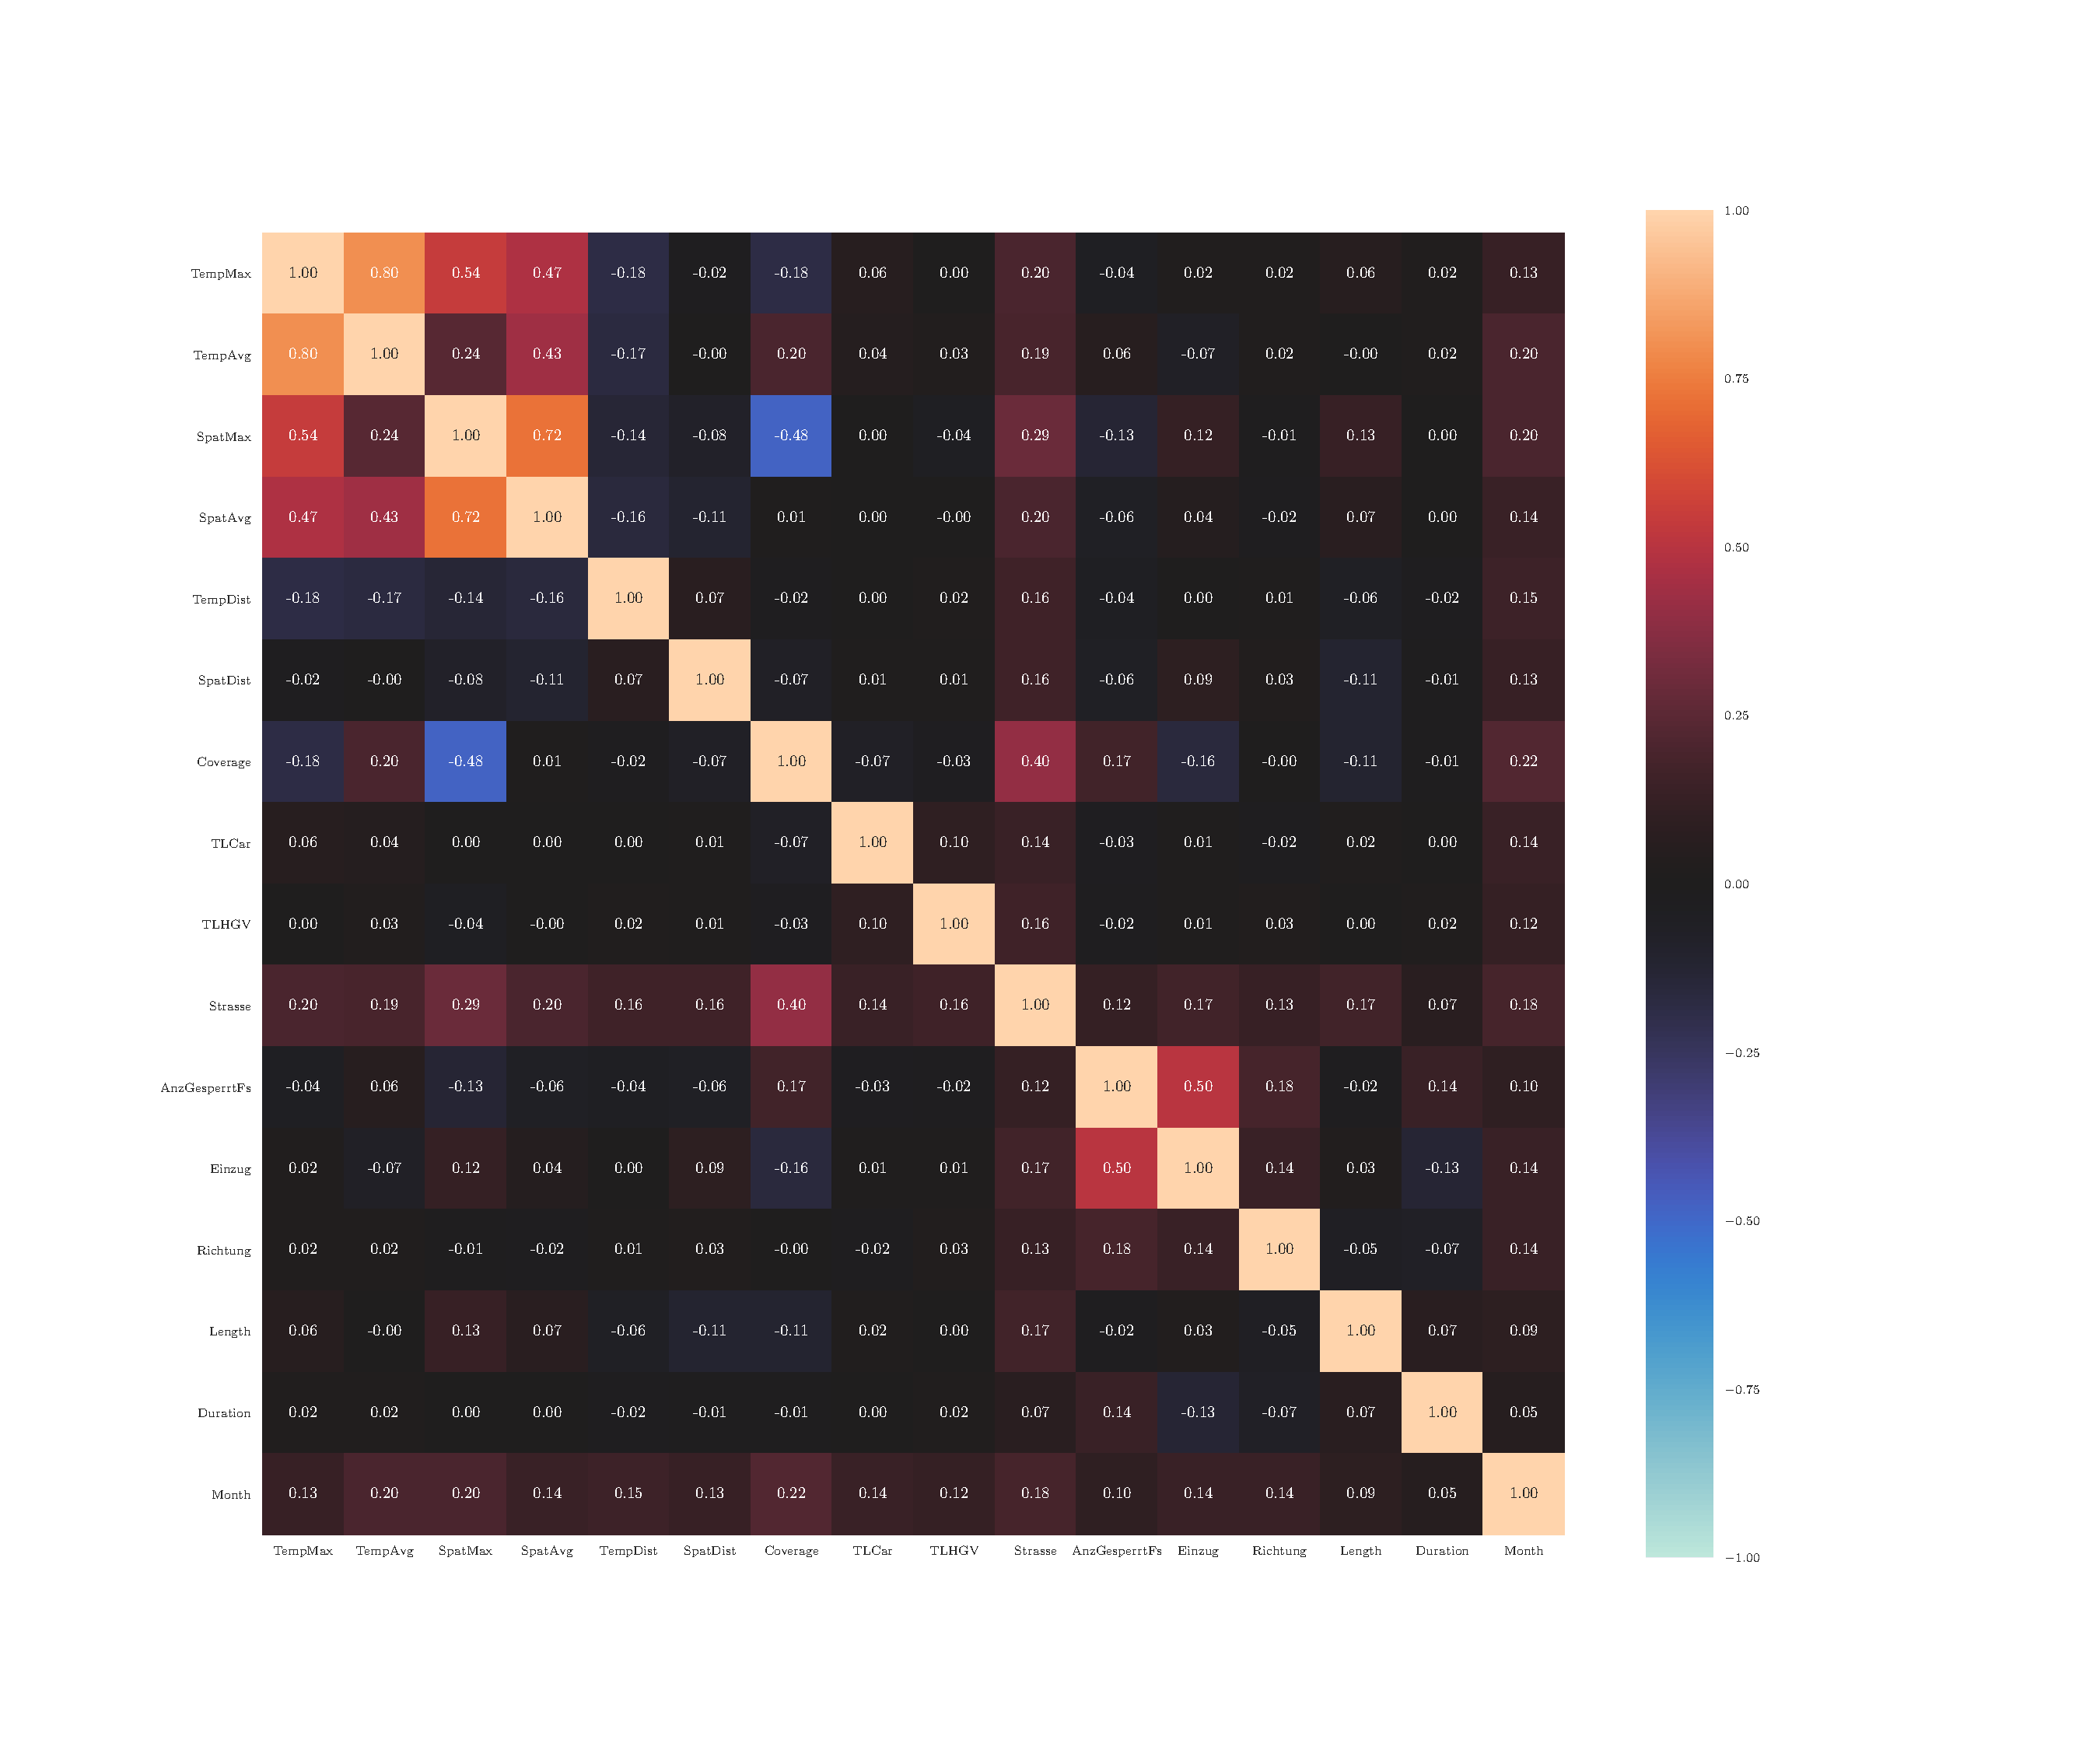
\includegraphics[width=1.4\textwidth, trim=0cm 2.5cm 6cm 3cm]{CorrAnalysis/data/ArbIS/02_matched/plots/arbis_matched_corr_cramers}%
	}
	\caption{Correlation matrix for congestion-roadwork matched data, calculated with $V$, $\eta$, $\tau$, $r_{pq}$, $r$}
	\label{img:correlation_matrix_arbis_selected_effector_cramers}
\end{figure}

% % --------------------------
% % -------- Strasse ---------
% % --------------------------
\centerheading{Strasse}
\varintrosimplewithsam{Strasse}

% ##############################################
\groupintrosigsig{Strasse}{TMax}{arbis}{matched}
\begin{table}[ht!]
	\tiny
	\centering
    \begin{tabular}{rrrrrrrrrrrrrrrrr}
		\toprule
			& A9 & A7 & A70 & A71 & A6 & A73 & A3 & A99 & A96 & A995 & A92 & A72 & A93 & A95 & A94 & A980 \\ 
		\midrule
		% A7   & 1.00 &  &  &  &  &  &  &  &  &  &  &  &  &  &  &  \\ 
		% A70  & 1.00 & 1.00 &  &  &  &  &  &  &  &  &  &  &  &  &  &  \\ 
		% A71  & 1.00 & 1.00 & 1.00 &  &  &  &  &  &  &  &  &  &  &  &  &  \\ 
		% A6   & 1.00 & 1.00 & 1.00 & 1.00 &  &  &  &  &  &  &  &  &  &  &  &  \\ 
		% A73  & 1.00 & 1.00 & 1.00 & 1.00 & 1.00 &  &  &  &  &  &  &  &  &  &  &  \\ 
		A3   & \red{0.00} & \red{0.04} & 1.00 & 1.00 & \red{0.01} & 1.00 &  &  &  &  &  &  &  &  &  &  \\ 
		% A99  & 1.00 & 1.00 & 1.00 & 1.00 & 0.48 & 1.00 & 1.00 &  &  &  &  &  &  &  &  &  \\ 
		A96  & 1.00 & 0.82 & 1.00 & 1.00 & 1.00 & 1.00 & \red{0.00} & \red{0.00} &  &  &  &  &  &  &  &  \\ 
		% A995 & 1.00 & 1.00 & 1.00 & 1.00 & 1.00 & 1.00 & 0.79 & 0.74 & 1.00 &  &  &  &  &  &  &  \\ 
		% A92  & 1.00 & 1.00 & 1.00 & 1.00 & 1.00 & 1.00 & 1.00 & 1.00 & 1.00 & 1.00 &  &  &  &  &  &  \\ 
		% A72  & 1.00 & 1.00 & 1.00 & 1.00 & 1.00 & 1.00 & 1.00 & 1.00 & 1.00 & 1.00 & 1.00 &  &  &  &  &  \\ 
		A93  & \red{0.00} & \red{0.00} & 1.00 & 0.09 & \red{0.00} & \red{0.00} & 1.00 & 1.00 & \red{0.00} & \red{0.00} & \red{0.00} & 1.00 &  &  &  &  \\ 
		% A95  & 1.00 & 1.00 & 1.00 & 1.00 & 1.00 & 1.00 & 1.00 & 1.00 & 1.00 & 1.00 & 1.00 & 1.00 & 1.00 &  &  &  \\ 
		A94  & 1.00 & 1.00 & 1.00 & 1.00 & 0.68 & 1.00 & 1.00 & 1.00 & \red{0.01} & 0.48 & 1.00 & 1.00 & 1.00 & 1.00 &  &  \\ 
		% A980 & 1.00 & 1.00 & 1.00 & 1.00 & 1.00 & 1.00 & 1.00 & 1.00 & 1.00 & 1.00 & 1.00 & 1.00 & 1.00 & 1.00 & 1.00 &  \\ 
		% A45  & 1.00 & 1.00 & 1.00 & 1.00 & 1.00 & 1.00 & 1.00 & 1.00 & 1.00 & 1.00 & 1.00 & 1.00 & 1.00 & 1.00 & 1.00 & 1.00 \\ 
		\bottomrule
	\end{tabular}
	\caption{Pairwise Wilcoxon $T$-test for \textit{Strasse} and \textit{Maximal Temporal Extent}}
	\label{tbl:wilcoxon_arbis_matched_Strasse_TMax}
\end{table}
The table shows, that the groups A3 and A93 differ from group A9, A7 and A6. The A93 also differs from A96, A995 and A92. The A96 differs from A3 and A99.
% #### START: Table and Plot
\pgfplotstableread[col sep=comma,header=false]{
	A9   , 656  , 159.55 , 175.78 , 100.50 , 9   , 1323 , 1314
	A7   , 302  , 158.38 , 213.55 , 87.00  , 9   , 1323 , 1314
	A70  , 50   , 228.90 , 279.03 , 105.00 , 15  , 963  , 948 
	A71  , 10   , 83.40  , 72.87  , 48.00  , 36  , 249  , 213 
	A6   , 198  , 142.24 , 166.46 , 85.50  , 9   , 864  , 855 
	A73  , 86   , 153.59 , 235.85 , 100.50 , 9   , 1323 , 1314
	A3   , 1023 , 233.66 , 279.35 , 123.00 , 9   , 1326 , 1317
	A99  , 312  , 158.88 , 155.05 , 135.00 , 9   , 1320 , 1311
	A96  , 230  , 105.80 , 95.17  , 75.00  , 9   , 384  , 375 
	A995 , 14   , 60.00  , 28.70  , 48.00  , 18  , 105  , 87 
	A92  , 82   , 132.40 , 134.72 , 79.50  , 9   , 768  , 759 
	A93  , 160  , 157.33 , 55.97  , 189.00 , 9   , 312  , 303 
	A94  , 56   , 179.57 , 124.79 , 165.00 , 15  , 369  , 354 
}\data
\pgfplotstablecreatecol[
  create col/expr={\thisrow{1} + \thisrow{2} + \thisrow{3} + \thisrow{4}}
]{sum}{\data}
\begin{figure}[ht!]
	\centering
	\begin{minipage}{0.5\textwidth}
		\tiny
		\setlength{\tabcolsep}{4pt}
		\centering
		\begin{tabular}{c|c|c|c|c|c|c|c}
			\toprule
			Group & $n$ & $\bar{x}$ & $\sigma$ & $\tilde{x}$ & $min$ & $max$ & $\Delta$ \\
			\midrule
			A9   & 656  & 159.55 & 175.78 & 100.50 & 9   & 1323 & 1314 \\ 
			A7   & 302  & 158.38 & 213.55 & 87.00  & 9   & 1323 & 1314 \\ 
			A70  & 50   & 228.90 & 279.03 & 105.00 & 15  & 963  & 948 \\ 
			A71  & 10   & 83.40  & 72.87  & 48.00  & 36  & 249  & 213 \\ 
			A6   & 198  & 142.24 & 166.46 & 85.50  & 9   & 864  & 855 \\ 
			A73  & 86   & 153.59 & 235.85 & 100.50 & 9   & 1323 & 1314 \\ 
			A3   & 1023 & 233.66 & 279.35 & 123.00 & 9   & 1326 & 1317 \\ 
			A99  & 312  & 158.88 & 155.05 & 135.00 & 9   & 1320 & 1311 \\ 
			A96  & 230  & 105.80 & 95.17  & 75.00  & 9   & 384  & 375 \\ 
			A995 & 14   & 60.00  & 28.70  & 48.00  & 18  & 105  & 87 \\ 
			A92  & 82   & 132.40 & 134.72 & 79.50  & 9   & 768  & 759 \\ 
			A93  & 160  & 157.33 & 55.97  & 189.00 & 9   & 312  & 303 \\  
			A94  & 56   & 179.57 & 124.79 & 165.00 & 15  & 369  & 354 \\ 
			\bottomrule
			% \bar{x} - sum = 1953.7, mean = 150.28
			% \sigma - sum = 2017.29, mean = 155.17
			% \tilde{x} 
		\end{tabular}
		\subcaption[second caption.]{Table of all descriptives}\label{tbl:descriptives_arbis_matched_Strasse_TMax}
	\end{minipage}%
	\begin{minipage}{0.55\textwidth}
		\tiny
		\centering
		% https://texwelt.de/fragen/26286/zwei-gruppen-bei-einem-gestapelten-balkendiagramm-und-zentrierte-balkenbeschriftungen
		% https://tex.stackexchange.com/questions/275229/forcing-all-axis-labels-to-display-in-a-plot
		\begin{tikzpicture}
			\begin{axis}[
				% Gitterlinien für y-Ticks
				width=\textwidth,
				height=5.5cm,
				xmajorgrids=true,
				ymajorgrids=true,
				xtick=data,
				xmin=0,xmax=12,
				xticklabels from table={\data}{[index]0},
				% zusätzliche Beschriftung an y-Achse
				every extra y tick/.style={
					tick0/.initial=blue,
					tick1/.initial=red,
					yticklabel style={
						color=\pgfkeysvalueof{/pgfplots/tick\ticknum}
					},
				},
				extra y ticks={150,155},
			]
			\addplot table [absolute series=2] {\data};
			\addplot table [absolute series=3] {\data};
			\addplot table [absolute series=4] {\data};
			\legend{
				$\bar{x}$,$\sigma$,$\tilde{x}$}
			\end{axis}
		 \end{tikzpicture}\vfill
		\subcaption[second caption.]{Plot of descriptives $\bar{x}$, $\sigma$ and $\tilde{x}$}\label{fig:descriptives_arbis_matched_Strasse_TMax}
	\end{minipage}%
	\caption{Group descriptives of \textit{Strasse} and \textit{Maximal Temporal Extent}}
	%\vspace{-8mm}
\end{figure}
% #### END: Table and Plot
With the descriptives in \cref{tbl:descriptives_arbis_matched_Strasse_TMax} and the named significant differences it can be interpreted that roadworks on the A3 result in 80\,\% longer $\bar{x}$ than on the A9, A7 and A6. The A70 has a similar difference. Roadworks on the A96 and A995 result in significantly shorter $\bar{x}$ than on the A3 and A99.

% ##############################################
\groupintrosigsig{Strasse}{TAvg}{arbis}{matched}
\begin{table}[ht!]
	\tiny
	\setlength{\tabcolsep}{4pt}
	\centering
	\begin{tabular}{rrrrrrrrrrrrrrrrr}
		\toprule
			& A9 & A7 & A70 & A71 & A6 & A73 & A3 & A99 & A96 & A995 & A92 & A72 & A93 & A95 & A94 & A980 \\ 
		\midrule
		% A7   & 1.00 &  &  &  &  &  &  &  &  &  &  &  &  &  &  &  \\ 
		% A70  & 1.00 & 1.00 &  &  &  &  &  &  &  &  &  &  &  &  &  &  \\ 
		% A71  & 1.00 & 1.00 & 1.00 &  &  &  &  &  &  &  &  &  &  &  &  &  \\ 
		% A6   & 1.00 & 1.00 & 1.00 & 1.00 &  &  &  &  &  &  &  &  &  &  &  &  \\ 
		% A73  & 1.00 & 1.00 & 1.00 & 1.00 & 1.00 &  &  &  &  &  &  &  &  &  &  &  \\ 
		% A3   & 1.00 & 1.00 & 1.00 & 1.00 & 0.69 & 1.00 &  &  &  &  &  &  &  &  &  &  \\ 
		A99  & \red{0.00} & \red{0.00} & 0.08 & 1.00 & 1.00 & 1.00 & \red{0.00} &  &  &  &  &  &  &  &  &  \\ 
		% A96  & 1.00 & 1.00 & 1.00 & 1.00 & 1.00 & 1.00 & 1.00 & 0.55 &  &  &  &  &  &  &  &  \\ 
		% A995 & 1.00 & 1.00 & 1.00 & 1.00 & 1.00 & 1.00 & 1.00 & 1.00 & 1.00 &  &  &  &  &  &  &  \\ 
		A92  & 1.00 & 1.00 & 1.00 & 1.00 & 1.00 & 1.00 & 1.00 & \red{0.04} & 1.00 & 1.00 &  &  &  &  &  &  \\ 
		% A72  & 1.00 & 1.00 & 1.00 & 1.00 & 1.00 & 1.00 & 1.00 & 1.00 & 1.00 & 1.00 & 1.00 &  &  &  &  &  \\ 
		A93  & \red{0.00} & \red{0.00} & 1.00 & 0.24 & \red{0.00} & \red{0.00} & \red{0.00} & \red{0.00} & \red{0.00} & \red{0.00} & \red{0.00} & 1.00 &  &  &  &  \\ 
		% A95  & 1.00 & 1.00 & 1.00 & 1.00 & 1.00 & 1.00 & 1.00 & 1.00 & 1.00 & 1.00 & 1.00 & 1.00 & 1.00 &  &  &  \\ 
		A94  & 1.00 & 1.00 & 1.00 & 1.00 & 0.14 & 1.00 & 1.00 & \red{0.00} & 0.63 & 0.53 & 1.00 & 1.00 & \red{0.02} & 1.00 &  &  \\ 
		% A980 & 1.00 & 1.00 & 1.00 & 1.00 & 1.00 & 1.00 & 1.00 & 1.00 & 1.00 & 1.00 & 1.00 & 1.00 & 1.00 & 1.00 & 1.00 &  \\ 
		% A45  & 1.00 & 1.00 & 1.00 & 1.00 & 1.00 & 1.00 & 1.00 & 1.00 & 1.00 & 1.00 & 1.00 & 1.00 & 1.00 & 1.00 & 1.00 & 1.00 \\ 
		\midrule
	\end{tabular}
	\caption{Pairwise Wilcoxon $T$-test for \textit{Strasse} and \textit{Average Temporal Extent}}
	\label{tbl:wilcoxon_arbis_matched_Strasse_TAvg}
\end{table}
The table shows, that the groups A99 and A93 differ from group A9 and A7. The A93 also differs from the A6, A73, A3, A99, A96, A995 and A92. The A92 differs from A99 and A99 from A3. The A94 differs from the A99 and A93.
% #### START: Table and Plot
\pgfplotstableread[col sep=comma,header=false]{
	A9   , 656  , 85.61  , 100.78 , 42.00  , 5  , 575  , 570  
	A7   , 302  , 87.76  , 117.13 , 44.50  , 5  , 858  , 853  
	A70  , 50   , 154.38 , 236.49 , 55.50  , 6  , 966  , 960  
	A71  , 10   , 64.90  , 71.81  , 38.00  , 18 , 252  , 234  
	A6   , 198  , 65.60  , 86.36  , 41.00  , 4  , 630  , 626  
	A73  , 86   , 56.23  , 45.35  , 42.50  , 6  , 190  , 184  
	A3   , 1023 , 89.94  , 124.69 , 51.00  , 3  , 1326 , 1323 
	A99  , 312  , 45.38  , 41.73  , 33.00  , 3  , 291  , 288  
	A96  , 230  , 69.31  , 73.52  , 43.00  , 5  , 290  , 285  
	A995 , 14   , 37.14  , 23.98  , 23.00  , 8  , 74   , 66 
	A92  , 82   , 81.83  , 90.35  , 45.50  , 5  , 489  , 484  
	A93  , 160  , 115.96 , 50.96  , 141.00 , 6  , 199  , 193  
	A94  , 56   , 84.98  , 64.07  , 70.00  , 6  , 248  , 242  
}\data
\pgfplotstablecreatecol[
  create col/expr={\thisrow{1} + \thisrow{2} + \thisrow{3} + \thisrow{4}}
]{sum}{\data}
\begin{figure}[ht!]
	\centering
	\begin{minipage}{0.5\textwidth}
		\tiny
		\setlength{\tabcolsep}{4pt}
		\centering
		\begin{tabular}{c|c|c|c|c|c|c|c}
			\toprule
			Group & $n$ & $\bar{x}$ & $\sigma$ & $\tilde{x}$ & $min$ & $max$ & $\Delta$ \\
			\midrule
			A9   & 656  & 85.61  & 100.78 & 42.00  & 5  & 575  & 570 \\ 
			A7   & 302  & 87.76  & 117.13 & 44.50  & 5  & 858  & 853 \\ 
			A70  & 50   & 154.38 & 236.49 & 55.50  & 6  & 966  & 960 \\ 
			A71  & 10   & 64.90  & 71.81  & 38.00  & 18 & 252  & 234 \\ 
			A6   & 198  & 65.60  & 86.36  & 41.00  & 4  & 630  & 626 \\ 
			A73  & 86   & 56.23  & 45.35  & 42.50  & 6  & 190  & 184 \\ 
			A3   & 1023 & 89.94  & 124.69 & 51.00  & 3  & 1326 & 1323 \\ 
			A99  & 312  & 45.38  & 41.73  & 33.00  & 3  & 291  & 288 \\ 
			A96  & 230  & 69.31  & 73.52  & 43.00  & 5  & 290  & 285 \\ 
			A995 & 14   & 37.14  & 23.98  & 23.00  & 8  & 74   & 66 \\ 
			A92  & 82   & 81.83  & 90.35  & 45.50  & 5  & 489  & 484 \\ 
			A93  & 160  & 115.96 & 50.96  & 141.00 & 6  & 199  & 193 \\ 
			A94  & 56   & 84.98  & 64.07  & 70.00  & 6  & 248  & 242 \\ 
			\bottomrule
			% \bar{x} - sum = 1039.02 mean = 79.92
			% \sigma - sum = 1127.22, mean = 86.70
			% \tilde{x} 
		\end{tabular}
		\subcaption[second caption.]{Table of all descriptives}\label{tbl:descriptives_arbis_matched_Strasse_TAvg}
	\end{minipage}%
	\begin{minipage}{0.55\textwidth}
		\tiny
		\centering
		\begin{tikzpicture}
			\begin{axis}[
				% Gitterlinien für y-Ticks
				width=\textwidth,
				height=5.5cm,
				xmajorgrids=true,
				ymajorgrids=true,
				xtick=data,
				xmin=0,xmax=12,
				% xticklabels={A9,A7,A70,A71,A6,A73,A3,A99,A96,A995,A92,A93,A94},
				xticklabels from table={\data}{[index]0},
				% zusätzliche Beschriftung an y-Achse
				every extra y tick/.style={
					tick0/.initial=blue,
					tick1/.initial=red,
					yticklabel style={
						color=\pgfkeysvalueof{/pgfplots/tick\ticknum}
					},
				},
				extra y ticks={80,87},
			]
			\addplot table [absolute series=2] {\data};
			\addplot table [absolute series=3] {\data};
			\addplot table [absolute series=4] {\data};
			\legend{
				$\bar{x}$,$\sigma$,$\tilde{x}$}
			\end{axis}
		 \end{tikzpicture}\vfill
		\subcaption[second caption.]{Plot of descriptives $\bar{x}$, $\sigma$ and $\tilde{x}$}\label{fig:descriptives_arbis_matched_Strasse_TAvg}
	\end{minipage}%
	\caption{Group descriptives of \textit{Strasse} and \textit{Average Temporal Extent}}
	%\vspace{-8mm}
\end{figure}
% #### END: Table and Plot
With the descriptives in \cref{tbl:descriptives_arbis_matched_Strasse_TAvg,fig:descriptives_arbis_matched_Strasse_TAvg} it can be interpreted that roadworks on the A73, A93, A99 and A995 result in significantly shorter jams than on the A3, A7, A70, A92 and A94. 

% ##############################################
\groupintrosigsig{Strasse}{SMax}{arbis}{matched}
\begin{table}[ht!]
	\tiny
	\setlength{\tabcolsep}{4pt}
	\centering
	\begin{tabular}{rrrrrrrrrrrrrrrrr}
		\toprule
			& A9 & A7 & A70 & A71 & A6 & A73 & A3 & A99 & A96 & A995 & A92 & A72 & A93 & A95 & A94 & A980 \\ 
		\midrule
		% A7   & 0.58 &  &  &  &  &  &  &  &  &  &  &  &  &  &  &  \\ 
		% A70  & 1.00 & 1.00 &  &  &  &  &  &  &  &  &  &  &  &  &  &  \\ 
		% A71  & 1.00 & 1.00 & 1.00 &  &  &  &  &  &  &  &  &  &  &  &  &  \\ 
		% A6   & 1.00 & 1.00 & 1.00 & 1.00 &  &  &  &  &  &  &  &  &  &  &  &  \\ 
		% A73  & 1.00 & 1.00 & 1.00 & 1.00 & 1.00 &  &  &  &  &  &  &  &  &  &  &  \\ 
		A3   & \red{0.00} & \red{0.00} & \red{0.00} & 0.52 & \red{0.01} & \red{0.05} &  &  &  &  &  &  &  &  &  &  \\ 
		% A99  & 0.07 & 0.00 & 0.01 & 0.21 & 0.26 & 0.20 & 1.00 &  &  &  &  &  &  &  &  &  \\ 
		A96  & \red{0.00} & 0.06 & 1.00 & 1.00 & 0.00 & 1.00 & \red{0.00} & \red{0.00} &  &  &  &  &  &  &  &  \\ 
		A995 & 1.00 & 1.00 & 1.00 & 1.00 & 1.00 & 1.00 & 0.11 & \red{0.03} & 1.00 &  &  &  &  &  &  &  \\ 
		A92  & 1.00 & 1.00 & 1.00 & 1.00 & 1.00 & 1.00 & \red{0.00} & \red{0.00} & \red{0.04} & 1.00 &  &  &  &  &  &  \\ 
		% A72  & 1.00 & 1.00 & 1.00 & 1.00 & 1.00 & 1.00 & 1.00 & 1.00 & 1.00 & 0.81 & 1.00 &  &  &  &  &  \\ 
		A93  & \red{0.00} & \red{0.00} & \red{0.02} & 1.00 & \red{0.00} & \red{0.00} & \red{0.00} & \red{0.00} & \red{0.00} & 1.00 & \red{0.00} & 0.73 &  &  &  &  \\ 
		% A95  & 1.00 & 1.00 & 1.00 & 1.00 & 1.00 & 1.00 & 1.00 & 1.00 & 1.00 & 1.00 & 1.00 & 1.00 & 1.00 &  &  &  \\ 
		A94  & 1.00 & 1.00 & 1.00 & 1.00 & 1.00 & 1.00 & \red{0.04} & \red{0.04} & 0.89 & 1.00 & 1.00 & 1.00 & \red{0.00} & 1.00 &  &  \\ 
		% A980 & 1.00 & 1.00 & 1.00 & 1.00 & 1.00 & 1.00 & 1.00 & 1.00 & 1.00 & 1.00 & 1.00 & 1.00 & 1.00 & 1.00 & 1.00 &  \\ 
		% A45  & 1.00 & 1.00 & 1.00 & 1.00 & 1.00 & 1.00 & 1.00 & 1.00 & 1.00 & 1.00 & 1.00 & 1.00 & 1.00 & 1.00 & 1.00 & 1.00 \\ 
		\bottomrule
	\end{tabular}
	\caption{Pairwise Wilcoxon $T$-test for \textit{Strasse} and \textit{Maximal Spatial Extent}}
	\label{tbl:wilcoxon_arbis_matched_Strasse_SMax}
\end{table}
The table shows, that the groups A3 and A93 differ from group A6, A7, A70, A73, A9, A96, A92, A93 and A94. The group A99 also differs from A96, A995, A92, A93 and A94. The A94 also differs from A99.
% #### START: Table and Plot
\pgfplotstableread[col sep=comma,header=false]{
	A9   , 656  , 8655.57  , 8521.51  , 4778 , 1035 , 49765 , 48730 
	A7   , 302  , 6238.63  , 4902.30  , 4397 , 902  , 20030 , 19128 
	A70  , 50   , 5729.56  , 4763.20  , 3224 , 1365 , 20249 , 18884 
	A71  , 10   , 3899.00  , 2746.84  , 2339 , 2075 , 10225 , 8150  
	A6   , 198  , 8421.67  , 8209.85  , 5690 , 965  , 40033 , 39068 
	A73  , 86   , 7717.21  , 7747.18  , 4813 , 1095 , 33764 , 32669 
	A3   , 1023 , 11836.50 , 11045.29 , 7979 , 1014 , 47607 , 46593 
	A99  , 312  , 9337.49  , 7230.99  , 7978 , 991  , 48987 , 47996 
	A96  , 230  , 5639.41  , 6034.92  , 3072 , 951  , 27965 , 27014 
	A995 , 14   , 3618.14  , 1331.10  , 4288 , 1613 , 4825  , 3212  
	A92  , 82   , 5758.10  , 3673.73  , 4544 , 999  , 16931 , 15932 
	A93  , 160  , 3530.39  , 3718.54  , 1926 , 99   , 22528 , 21829 
	A94  , 56   , 5849.05  , 3394.57  , 5785 , 1025 , 12582 , 11557 
}\data
\pgfplotstablecreatecol[
  create col/expr={\thisrow{1} + \thisrow{2} + \thisrow{3} + \thisrow{4}}
]{sum}{\data}
\begin{figure}[ht!]
	\centering
	\begin{minipage}{0.5\textwidth}
		\tiny
		\setlength{\tabcolsep}{4pt}
		\centering
		\begin{tabular}{c|c|c|c|c|c|c|c}
			\toprule
			Group & $n$ & $\bar{x}$ & $\sigma$ & $\tilde{x}$ & $min$ & $max$ & $\Delta$ \\
			\midrule
			A9   & 656  & 8655.57  & 8521.51  & 4778 & 1035 & 49765 & 48730 \\ 
			A7   & 302  & 6238.63  & 4902.30  & 4397 & 902  & 20030 & 19128 \\ 
			A70  & 50   & 5729.56  & 4763.20  & 3224 & 1365 & 20249 & 18884 \\ 
			A71  & 10   & 3899.00  & 2746.84  & 2339 & 2075 & 10225 & 8150  \\ 
			A6   & 198  & 8421.67  & 8209.85  & 5690 & 965  & 40033 & 39068 \\ 
			A73  & 86   & 7717.21  & 7747.18  & 4813 & 1095 & 33764 & 32669 \\ 
			A3   & 1023 & 11836.50 & 11045.29 & 7979 & 1014 & 47607 & 46593 \\ 
			A99  & 312  & 9337.49  & 7230.99  & 7978 & 991  & 48987 & 47996 \\ 
			A96  & 230  & 5639.41  & 6034.92  & 3072 & 951  & 27965 & 27014 \\ 
			A995 & 14   & 3618.14  & 1331.10  & 4288 & 1613 & 4825  & 3212  \\ 
			A92  & 82   & 5758.10  & 3673.73  & 4544 & 999  & 16931 & 15932 \\ 
			A93  & 160  & 3530.39  & 3718.54  & 1926 & 99   & 22528 & 21829 \\ 
			A94  & 56   & 5849.05  & 3394.57  & 5785 & 1025 & 12582 & 11557 \\ 
			\bottomrule
			% \bar{x} - sum = 80230.72, mean = 6633.13 
			% \sigma - sum = 73320.02, mean = 5640.00
			% \tilde{x} 
		\end{tabular}
		\subcaption[second caption.]{Table of all descriptives}\label{tbl:descriptives_arbis_matched_Strasse_SMax}
	\end{minipage}%
	\begin{minipage}{0.55\textwidth}
		\tiny
		\centering
		\begin{tikzpicture}
			\begin{axis}[
				width=\textwidth,
				height=5.5cm,
				xmajorgrids=true,
				ymajorgrids=true,
				xtick=data,
				xmin=0,xmax=12,
				xticklabels from table={\data}{[index]0},
				% zusätzliche Beschriftung an y-Achse
				every extra y tick/.style={
					tick0/.initial=blue,
					tick1/.initial=red,
					yticklabel style={
						color=\pgfkeysvalueof{/pgfplots/tick\ticknum}
					},
				},
				extra y ticks={6633,5640},
				extra y tick labels={0.6,0.5}
			]
			\addplot table [absolute series=2] {\data};
			\addplot table [absolute series=3] {\data};
			\addplot table [absolute series=4] {\data};
			\legend{
				$\bar{x}$,$\sigma$,$\tilde{x}$}
			\end{axis}
		 \end{tikzpicture}\vfill
		\subcaption[second caption.]{Plot of descriptives $\bar{x}$, $\sigma$ and $\tilde{x}$}\label{fig:descriptives_arbis_matched_Strasse_SMax}
	\end{minipage}%
	\caption{Group descriptives of \textit{Strasse} and \textit{Maximal Spatial Extent}}
	%\vspace{-8mm}
\end{figure}
% #### END: Table and Plot
With the descriptives in \cref{tbl:descriptives_arbis_matched_Strasse_SMax,fig:descriptives_arbis_matched_Strasse_SMax} it can be interpreted that roadworks on the A3, A9, A6 A99 and A73 result in significantly longer jams than on the A96, A92, A94, A93 and A70.

% ##############################################
\groupintrosigsig{Strasse}{SAvg}{arbis}{matched}
\begin{table}[ht!]
	\tiny
	\setlength{\tabcolsep}{4pt}
	\centering
	\begin{tabular}{rrrrrrrrrrrrrrrrr}
		\toprule
			& A9 & A7 & A70 & A71 & A6 & A73 & A3 & A99 & A96 & A995 & A92 & A72 & A93 & A95 & A94 & A980 \\ 
		\midrule
		% A7   & 0.06 &  &  &  &  &  &  &  &  &  &  &  &  &  &  &  \\ 
		% A70  & 1.00 & 1.00 &  &  &  &  &  &  &  &  &  &  &  &  &  &  \\ 
		% A71  & 1.00 & 1.00 & 1.00 &  &  &  &  &  &  &  &  &  &  &  &  &  \\ 
		% A6   & 1.00 & 1.00 & 1.00 & 1.00 &  &  &  &  &  &  &  &  &  &  &  &  \\ 
		% A73  & 0.62 & 1.00 & 1.00 & 1.00 & 1.00 &  &  &  &  &  &  &  &  &  &  &  \\ 
		A3   & 1.00 & 0.00 & 1.00 & 1.00 & 1.00 & \red{0.02} &  &  &  &  &  &  &  &  &  &  \\ 
		A99  & \red{0.01} & 1.00 & 1.00 & 1.00 & 0.75 & 1.00 & \red{0.00} &  &  &  &  &  &  &  &  &  \\ 
		A96  & \red{0.00} & 1.00 & 1.00 & 1.00 & 0.44 & 1.00 & \red{0.00} & 1.00 &  &  &  &  &  &  &  &  \\ 
		% A995 & 1.00 & 1.00 & 1.00 & 1.00 & 1.00 & 1.00 & 1.00 & 1.00 & 1.00 &  &  &  &  &  &  &  \\ 
		% A92  & 1.00 & 0.62 & 1.00 & 1.00 & 1.00 & 0.73 & 1.00 & 0.10 & 0.14 & 1.00 &  &  &  &  &  &  \\ 
		% A72  & 1.00 & 1.00 & 1.00 & 1.00 & 1.00 & 1.00 & 1.00 & 1.00 & 1.00 & 1.00 & 1.00 &  &  &  &  &  \\ 
		A93  & \red{0.00} & 0.13 & 1.00 & 1.00 & 0.00 & 1.00 & \red{0.00} & 0.11 & 1.00 & 1.00 & \red{0.00} & 1.00 &  &  &  &  \\ 
		% A95  & 1.00 & 1.00 & 1.00 & 1.00 & 1.00 & 1.00 & 1.00 & 1.00 & 1.00 & 1.00 & 1.00 & 1.00 & 1.00 &  &  &  \\ 
		% A94  & 1.00 & 1.00 & 1.00 & 1.00 & 1.00 & 1.00 & 1.00 & 1.00 & 1.00 & 1.00 & 1.00 & 1.00 & 1.00 & 1.00 &  &  \\ 
		% A980 & 1.00 & 1.00 & 1.00 & 1.00 & 1.00 & 1.00 & 1.00 & 1.00 & 1.00 & 1.00 & 1.00 & 1.00 & 1.00 & 1.00 & 1.00 &  \\ 
		% A45  & 1.00 & 1.00 & 1.00 & 1.00 & 1.00 & 1.00 & 1.00 & 1.00 & 1.00 & 1.00 & 1.00 & 1.00 & 1.00 & 1.00 & 1.00 & 1.00 \\ 
		\bottomrule
	\end{tabular}
	\caption{Pairwise Wilcoxon $T$-test for \textit{Strasse} and \textit{Average Spatial Extent}}
	\label{tbl:wilcoxon_arbis_matched_Strasse_SAvg}
\end{table}
It shows, that the groups A99, A96 and A93 differ from group A9 and A3. The A93 also differs from A92 and A73 from A3.
% #### START: Table and Plot
\pgfplotstableread[col sep=comma,header=false]{
	A9   , 656  , 3537.87 , 3014.80 , 2388.50 , 697 , 14785 , 14088 
	A7   , 302  , 2917.97 , 2988.99 , 2113.50 , 284 , 15602 , 15318 
	A70  , 50   , 3170.10 , 3033.98 , 1816.00 , 532 , 12543 , 12011 
	A71  , 10   , 2572.50 , 3027.05 , 1323.00 , 802 , 10425 , 9623  
	A6   , 198  , 3189.79 , 2385.78 , 2267.00 , 458 , 14150 , 13692 
	A73  , 86   , 2508.40 , 1834.03 , 2006.00 , 419 , 10039 , 9620  
	A3   , 1023 , 3733.90 , 2979.43 , 2835.00 , 355 , 15054 , 14699 
	A99  , 312  , 2381.29 , 1265.40 , 1974.00 , 502 , 5931  , 5429  
	A96  , 230  , 2488.22 , 1790.94 , 2160.00 , 404 , 9767  , 9363  
	A995 , 14   , 1976.93 , 1044.51 , 1950.00 , 569 , 3196  , 2627  
	A92  , 82   , 3360.88 , 2294.30 , 2882.00 , 457 , 11703 , 11246 
	A93  , 160  , 2243.26 , 2065.34 , 1575.00 , 461 , 11161 , 10700  
	A94  , 56   , 2557.62 , 1655.86 , 2551.00 , 506 , 6393  , 5887  
}\data
\pgfplotstablecreatecol[
  create col/expr={\thisrow{1} + \thisrow{2} + \thisrow{3} + \thisrow{4}}
]{sum}{\data}
\begin{figure}[ht!]
	\centering
	\begin{minipage}{0.5\textwidth}
		\tiny
		\setlength{\tabcolsep}{4pt}
		\centering
		\begin{tabular}{c|c|c|c|c|c|c|c}
			\toprule
			Group & $n$ & $\bar{x}$ & $\sigma$ & $\tilde{x}$ & $min$ & $max$ & $\Delta$ \\
			\midrule
			A9   & 656  & 3537.87 & 3014.80 & 2388.50 & 697 & 14785 & 14088 \\ 
			A7   & 302  & 2917.97 & 2988.99 & 2113.50 & 284 & 15602 & 15318 \\ 
			A70  & 50   & 3170.10 & 3033.98 & 1816.00 & 532 & 12543 & 12011 \\ 
			A71  & 10   & 2572.50 & 3027.05 & 1323.00 & 802 & 10425 & 9623  \\ 
			A6   & 198  & 3189.79 & 2385.78 & 2267.00 & 458 & 14150 & 13692 \\
			A73  & 86   & 2508.40 & 1834.03 & 2006.00 & 419 & 10039 & 9620  \\ 
			A3   & 1023 & 3733.90 & 2979.43 & 2835.00 & 355 & 15054 & 14699 \\ 
			A99  & 312  & 2381.29 & 1265.40 & 1974.00 & 502 & 5931  & 5429  \\ 
			A96  & 230  & 2488.22 & 1790.94 & 2160.00 & 404 & 9767  & 9363  \\ 
			A995 & 14   & 1976.93 & 1044.51 & 1950.00 & 569 & 3196  & 2627  \\ 
			A92  & 82   & 3360.88 & 2294.30 & 2882.00 & 457 & 11703 & 11246 \\ 
			A93  & 160  & 2243.26 & 2065.34 & 1575.00 & 461 & 11161 & 10700 \\  
			A94  & 56   & 2557.62 & 1655.86 & 2551.00 & 506 & 6393  & 5887  \\ 
			\bottomrule
			% \bar{x} - sum = 36638.73, mean = 2818.36 
			% \sigma - sum = 29380.41, mean = 2260.03
			% \tilde{x} 
		\end{tabular}
		\subcaption[second caption.]{Table of all descriptives}\label{tbl:descriptives_arbis_matched_Strasse_SAvg}
	\end{minipage}%
	\begin{minipage}{0.55\textwidth}
		\tiny
		\centering
		\begin{tikzpicture}
			\begin{axis}[
				width=\textwidth,
				height=5.5cm,
				xmajorgrids=true,
				ymajorgrids=true,
				xtick=data,
				xmin=0,xmax=12,
				xticklabels from table={\data}{[index]0},
				% zusätzliche Beschriftung an y-Achse
				every extra y tick/.style={
					tick0/.initial=blue,
					tick1/.initial=red,
					yticklabel style={
						color=\pgfkeysvalueof{/pgfplots/tick\ticknum}
					},
				},
				extra y ticks={2818,2260},
			]
			\addplot table [absolute series=2] {\data};
			\addplot table [absolute series=3] {\data};
			\addplot table [absolute series=4] {\data};
			\legend{
				$\bar{x}$,$\sigma$,$\tilde{x}$}
			\end{axis}
		 \end{tikzpicture}\vfill
		\subcaption[second caption.]{Plot of descriptives $\bar{x}$, $\sigma$ and $\tilde{x}$}\label{fig:descriptives_arbis_matched_Strasse_SAvg}
	\end{minipage}%
	\caption{Group descriptives of \textit{Strasse} and \textit{Average Spatial Extent}}
	%\vspace{-8mm}
\end{figure}
% #### END: Table and Plot
With the descriptives in \cref{tbl:descriptives_arbis_matched_Strasse_SAvg,fig:descriptives_arbis_matched_Strasse_SAvg} it can be interpreted that roadworks on the A3, A9 and A93 result in significantly longer jams than on the A92, A93, A96 and A73.

% ###############################################
\groupintrosigsig{Strasse}{TDist}{arbis}{matched}
\begin{table}[ht!]
	\tiny
	\setlength{\tabcolsep}{4pt}
	\centering
	\begin{tabular}{rrrrrrrrrrrrrrrrr}
		\toprule
			& A9 & A7 & A70 & A71 & A6 & A73 & A3 & A99 & A96 & A995 & A92 & A72 & A93 & A95 & A94 & A980 \\ 
		\midrule
		A7   & \red{0.00} &  &  &  &  &  &  &  &  &  &  &  &  &  &  &  \\ 
		% A70  & 0.57 & 1.00 &  &  &  &  &  &  &  &  &  &  &  &  &  &  \\ 
		% A71  & 1.00 & 1.00 & 1.00 &  &  &  &  &  &  &  &  &  &  &  &  &  \\ 
		% A6   & 0.10 & 1.00 & 1.00 & 1.00 &  &  &  &  &  &  &  &  &  &  &  &  \\ 
		% A73  & 1.00 & 1.00 & 1.00 & 1.00 & 1.00 &  &  &  &  &  &  &  &  &  &  &  \\ 
		A3   & \red{0.00} & 1.00 & 1.00 & 1.00 & 1.00 & 0.85 &  &  &  &  &  &  &  &  &  &  \\ 
		% A99  & 0.38 & 1.00 & 1.00 & 1.00 & 1.00 & 1.00 & 0.26 &  &  &  &  &  &  &  &  &  \\ 
		A96  & 1.00 & 1.00 & 1.00 & 1.00 & 1.00 & 1.00 & \red{0.03} & 1.00 &  &  &  &  &  &  &  &  \\ 
		% A995 & 1.00 & 1.00 & 1.00 & 1.00 & 1.00 & 1.00 & 1.00 & 1.00 & 1.00 &  &  &  &  &  &  &  \\ 
		A92  & \red{0.04} & 1.00 & 1.00 & 1.00 & 1.00 & 1.00 & 1.00 & 1.00 & 1.00 & 1.00 &  &  &  &  &  &  \\ 
		% A72  & 1.00 & 1.00 & 1.00 & 1.00 & 1.00 & 1.00 & 1.00 & 1.00 & 1.00 & 1.00 & 1.00 &  &  &  &  &  \\ 
		% A93  & 0.63 & 1.00 & 1.00 & 1.00 & 1.00 & 1.00 & 1.00 & 1.00 & 1.00 & 1.00 & 1.00 & 1.00 &  &  &  &  \\ 
		% A95  & 1.00 & 1.00 & 1.00 & 1.00 & 1.00 & 1.00 & 1.00 & 1.00 & 1.00 & 1.00 & 1.00 &  & 1.00 &  &  &  \\ 
		% A94  & 1.00 & 1.00 & 1.00 & 1.00 & 1.00 & 1.00 & 1.00 & 1.00 & 1.00 & 1.00 & 1.00 & 1.00 & 1.00 & 1.00 &  &  \\ 
		% A980 & 1.00 & 1.00 & 1.00 & 1.00 & 1.00 & 1.00 & 1.00 & 1.00 & 1.00 & 1.00 & 1.00 &  & 1.00 &  & 1.00 &  \\ 
		% A45  & 1.00 & 1.00 & 1.00 & 1.00 & 1.00 & 1.00 & 1.00 & 1.00 & 1.00 & 1.00 & 1.00 &  & 1.00 &  & 1.00 &  \\ 
		\bottomrule
	\end{tabular}
	\caption{Pairwise Wilcoxon $T$-test for \textit{Strasse} and \textit{Temporal Distance}}
	\label{tbl:wilcoxon_arbis_matched_Strasse_TDist}
\end{table}
It shows, that the groups A7, A3 and A92 differ from group A9. The A96 differs from the A3.
% #### START: Table and Plot
\pgfplotstableread[col sep=comma,header=false]{
	A9   , 656  , 4.12 , 7.16 , 0 , 0 , 24 , 24 
	A7   , 302  , 2.10 , 5.21 , 0 , 0 , 24 , 24 
	A70  , 50   , 1.64 , 5.20 , 0 , 0 , 23 , 23 
	A71  , 10   , 3.40 , 4.74 , 0 , 0 , 13 , 13 
	A6   , 198  , 2.09 , 5.07 , 0 , 0 , 23 , 23 
	A73  , 86   , 3.16 , 6.33 , 0 , 0 , 24 , 24 
	A3   , 1023 , 1.81 , 4.92 , 0 , 0 , 24 , 24 
	A99  , 312  , 2.72 , 5.91 , 0 , 0 , 24 , 24 
	A96  , 230  , 3.09 , 6.17 , 0 , 0 , 24 , 24 
	A995 , 14   , 1.64 , 6.15 , 0 , 0 , 23 , 23 
	A92  , 82   , 1.20 , 3.85 , 0 , 0 , 22 , 22 
	A93  , 160  , 2.39 , 5.50 , 0 , 0 , 23 , 23 
	A94  , 56   , 2.18 , 5.06 , 0 , 0 , 23 , 23 
}\data
\pgfplotstablecreatecol[
  create col/expr={\thisrow{1} + \thisrow{2} + \thisrow{3} + \thisrow{4}}
]{sum}{\data}
\begin{figure}[ht!]
	\centering
	\begin{minipage}{0.5\textwidth}
		\tiny
		% \setlength{\tabcolsep}{4pt}
		\centering
		\begin{tabular}{c|c|c|c|c|c|c|c}
			\toprule
			Group & $n$ & $\bar{x}$ & $\sigma$ & $\tilde{x}$ & $min$ & $max$ & $\Delta$ \\
			\midrule
			A9   & 656  & 4.12 & 7.16 & 0 & 0 & 24 & 24 \\ 
			A7   & 302  & 2.10 & 5.21 & 0 & 0 & 24 & 24 \\ 
			A70  & 50   & 1.64 & 5.20 & 0 & 0 & 23 & 23 \\ 
			A71  & 10   & 3.40 & 4.74 & 0 & 0 & 13 & 13 \\ 
			A6   & 198  & 2.09 & 5.07 & 0 & 0 & 23 & 23 \\ 
			A73  & 86   & 3.16 & 6.33 & 0 & 0 & 24 & 24 \\ 
			A3   & 1023 & 1.81 & 4.92 & 0 & 0 & 24 & 24 \\ 
			A99  & 312  & 2.72 & 5.91 & 0 & 0 & 24 & 24 \\ 
			A96  & 230  & 3.09 & 6.17 & 0 & 0 & 24 & 24 \\ 
			A995 & 14   & 1.64 & 6.15 & 0 & 0 & 23 & 23 \\ 
			A92  & 82   & 1.20 & 3.85 & 0 & 0 & 22 & 22 \\ 
			A93  & 160  & 2.39 & 5.50 & 0 & 0 & 23 & 23 \\ 
			A94  & 56   & 2.18 & 5.06 & 0 & 0 & 23 & 23 \\ 
			\bottomrule
			% \bar{x} - sum = 31.54, mean = 2.42 
			% \sigma - sum = 71.27, mean = 5.48
			% \tilde{x} 
		\end{tabular}
		\subcaption[second caption.]{Table of all descriptives}\label{tbl:descriptives_arbis_matched_Strasse_TDist}
	\end{minipage}%
	\begin{minipage}{0.55\textwidth}
		\tiny
		\centering
		\begin{tikzpicture}
			\begin{axis}[
				width=\textwidth,
				height=5.5cm,
				xmajorgrids=true,
				ymajorgrids=true,
				xtick=data,
				xmin=0,xmax=12,
				xticklabels from table={\data}{[index]0},
				% zusätzliche Beschriftung an y-Achse
				every extra y tick/.style={
					tick0/.initial=blue,
					tick1/.initial=red,
					yticklabel style={
						color=\pgfkeysvalueof{/pgfplots/tick\ticknum}
					},
				},
				extra y ticks={2.42,5.48},
			]
			\addplot table [absolute series=2] {\data};
			\addplot table [absolute series=3] {\data};
			\addplot table [absolute series=4] {\data};
			\legend{
				$\bar{x}$,$\sigma$,$\tilde{x}$}
			\end{axis}
		 \end{tikzpicture}\vfill
		\subcaption[second caption.]{Plot of descriptives $\bar{x}$, $\sigma$ and $\tilde{x}$}\label{fig:descriptives_arbis_matched_Strasse_TDist}
	\end{minipage}%
	\caption{Group descriptives of \textit{Strasse} and \textit{Temporal Distance}}
	%\vspace{-8mm}
\end{figure}
% #### END: Table and Plot
The descriptives in \cref{tbl:descriptives_arbis_matched_Strasse_TDist,fig:descriptives_arbis_matched_Strasse_TDist} don't show a clear interpretation, although the A9 shows a clear maximum and A92 a clear minimum.

% ###############################################
\groupintrosigsig{Strasse}{SDist}{arbis}{matched}
\begin{table}[ht!]
	\tiny
	\setlength{\tabcolsep}{4pt}
	\centering
	\begin{tabular}{rrrrrrrrrrrrrrrrr}
		\toprule
			& A9 & A7 & A70 & A71 & A6 & A73 & A3 & A99 & A96 & A995 & A92 & A72 & A93 & A95 & A94 & A980 \\ 
		\midrule
		% A7   & 0.62 &  &  &  &  &  &  &  &  &  &  &  &  &  &  &  \\ 
		% A70  & 1.00 & 1.00 &  &  &  &  &  &  &  &  &  &  &  &  &  &  \\ 
		% A71  & 1.00 & 1.00 & 1.00 &  &  &  &  &  &  &  &  &  &  &  &  &  \\ 
		% A6   & 1.00 & 1.00 & 1.00 & 1.00 &  &  &  &  &  &  &  &  &  &  &  &  \\ 
		A73  & \red{0.03} & 1.00 & 1.00 & 1.00 & 0.89 &  &  &  &  &  &  &  &  &  &  &  \\ 
		% A3   & 1.00 & 1.00 & 1.00 & 1.00 & 1.00 & 0.33 &  &  &  &  &  &  &  &  &  &  \\ 
		A99  & 1.00 & 0.61 & 1.00 & 1.00 & 1.00 & \red{0.03} & 1.00 &  &  &  &  &  &  &  &  &  \\ 
		% A96  & 1.00 & 1.00 & 1.00 & 1.00 & 1.00 & 1.00 & 1.00 & 1.00 &  &  &  &  &  &  &  &  \\ 
		% A995 & 1.00 & 1.00 & 1.00 & 1.00 & 1.00 & 1.00 & 1.00 & 1.00 & 1.00 &  &  &  &  &  &  &  \\ 
		% A92  & 1.00 & 1.00 & 1.00 & 1.00 & 1.00 & 1.00 & 1.00 & 1.00 & 1.00 & 1.00 &  &  &  &  &  &  \\ 
		% A72  & 1.00 & 1.00 & 1.00 & 1.00 & 1.00 & 1.00 & 1.00 & 1.00 & 1.00 & 1.00 & 1.00 &  &  &  &  &  \\ 
		A93  & \red{0.00} & \red{0.05} & 1.00 & 1.00 & 0.01 & 1.00 & \red{0.00} & \red{0.00} & 0.06 & 0.16 & 0.12 & 1.00 &  &  &  &  \\ 
		% A95  & 1.00 & 1.00 & 1.00 & 1.00 & 1.00 & 1.00 & 1.00 & 1.00 & 1.00 & 1.00 & 1.00 &  & 1.00 &  &  &  \\ 
		A94  & 1.00 & 0.09 & 0.72 & 1.00 & 0.76 & \red{0.00} & 0.40 & 1.00 & 0.30 & 1.00 & 1.00 & 1.00 & \red{0.00} & 1.00 &  &  \\ 
		% A980 & 1.00 & 1.00 & 1.00 & 1.00 & 1.00 & 1.00 & 1.00 & 1.00 & 1.00 & 1.00 & 1.00 &  & 1.00 &  & 1.00 &  \\ 
		% A45  & 1.00 & 1.00 & 1.00 & 1.00 & 1.00 & 1.00 & 1.00 & 1.00 & 1.00 & 1.00 & 1.00 & 1.00 & 1.00 & 1.00 & 1.00 & 1.00 \\ 
		\bottomrule
	\end{tabular}
	\caption{Pairwise Wilcoxon $T$-test for \textit{Strasse} and \textit{Spatial Distance}}
	\label{tbl:wilcoxon_arbis_matched_Strasse_SDist}
\end{table}
It shows that the groups A3, A73, A93, A94 and A99 differ significantly.
% #### START: Table and Plot
\pgfplotstableread[col sep=comma,header=false]{
	A9   , 656  , 216.54 , 466.13 , 0.00 , 0 , 1988 , 1988 
	A7   , 302  , 106.12 , 329.01 , 0.00 , 0 , 1882 , 1882 
	A70  , 50   , 72.94  , 257.26 , 0.00 , 0 , 1253 , 1253 
	A71  , 10   , 25.80  , 81.59  , 0.00 , 0 , 258  , 258  
	A6   , 198  , 130.20 , 379.68 , 0.00 , 0 , 1968 , 1968 
	A73  , 86   , 49.74  , 245.74 , 0.00 , 0 , 1924 , 1924 
	A3   , 1023 , 137.75 , 381.13 , 0.00 , 0 , 1979 , 1979 
	A99  , 312  , 260.51 , 542.02 , 0.00 , 0 , 1977 , 1977 
	A96  , 230  , 146.79 , 395.78 , 0.00 , 0 , 1958 , 1958 
	A995 , 14   , 288.29 , 545.94 , 0.00 , 0 , 1749 , 1749 
	A92  , 82   , 96.22  , 295.14 , 0.00 , 0 , 1626 , 1626 
	A93  , 160  , 34.58  , 189.72 , 0.00 , 0 , 1769 , 1769 
	A94  , 56   , 327.38 , 606.32 , 0.00 , 0 , 1983 , 1983  
}\data
\pgfplotstablecreatecol[
  create col/expr={\thisrow{1} + \thisrow{2} + \thisrow{3} + \thisrow{4}}
]{sum}{\data}
\begin{figure}[ht!]
	\centering
	\begin{minipage}{0.5\textwidth}
		\tiny
		% \setlength{\tabcolsep}{4pt}
		\centering
		\begin{tabular}{c|c|c|c|c|c|c|c}
			\toprule
			Group & $n$ & $\bar{x}$ & $\sigma$ & $\tilde{x}$ & $min$ & $max$ & $\Delta$ \\
			\midrule
			A9   & 656  & 216.54 & 466.13 & 0 & 0 & 1988 & 1988 \\ 
			A7   & 302  & 106.12 & 329.01 & 0 & 0 & 1882 & 1882 \\ 
			A70  & 50   & 72.94  & 257.26 & 0 & 0 & 1253 & 1253 \\ 
			A71  & 10   & 25.80  & 81.59  & 0 & 0 & 258  & 258  \\ 
			A6   & 198  & 130.20 & 379.68 & 0 & 0 & 1968 & 1968 \\ 
			A73  & 86   & 49.74  & 245.74 & 0 & 0 & 1924 & 1924 \\ 
			A3   & 1023 & 137.75 & 381.13 & 0 & 0 & 1979 & 1979 \\ 
			A99  & 312  & 260.51 & 542.02 & 0 & 0 & 1977 & 1977 \\ 
			A96  & 230  & 146.79 & 395.78 & 0 & 0 & 1958 & 1958 \\ 
			A995 & 14   & 288.29 & 545.94 & 0 & 0 & 1749 & 1749 \\ 
			A92  & 82   & 96.22  & 295.14 & 0 & 0 & 1626 & 1626 \\ 
			A93  & 160  & 34.58  & 189.72 & 0 & 0 & 1769 & 1769 \\ 
			A94  & 56   & 327.38 & 606.32 & 0 & 0 & 1983 & 1983 \\ 
			\bottomrule
			% \bar{x} - sum = 1982.86, mean = 145.60 
			% \sigma - sum = 4715.46, mean = 362.72
			% \tilde{x} 
		\end{tabular}
		\subcaption[second caption.]{Table of all descriptives}\label{tbl:descriptives_arbis_matched_Strasse_SDist}
	\end{minipage}%
	\begin{minipage}{0.55\textwidth}
		\tiny
		\centering
		\begin{tikzpicture}
			\begin{axis}[
				width=\textwidth,
				height=5.1cm,
				xmajorgrids=true,
				ymajorgrids=true,
				xtick=data,
				xmin=0,xmax=12,
				xticklabels from table={\data}{[index]0},
				% zusätzliche Beschriftung an y-Achse
				every extra y tick/.style={
					tick0/.initial=blue,
					tick1/.initial=red,
					yticklabel style={
						color=\pgfkeysvalueof{/pgfplots/tick\ticknum}
					},
				},
				extra y ticks={145,362},
			]
			\addplot table [absolute series=2] {\data};
			\addplot table [absolute series=3] {\data};
			\addplot table [absolute series=4] {\data};
			\legend{
				$\bar{x}$,$\sigma$,$\tilde{x}$}
			\end{axis}
		 \end{tikzpicture}\vfill
		\subcaption[second caption.]{Plot of descriptives $\bar{x}$, $\sigma$ and $\tilde{x}$}\label{fig:descriptives_arbis_matched_Strasse_SDist}
	\end{minipage}%
	\caption{Group descriptives of \textit{Strasse} and \textit{Spatial Distance}}
	%\vspace{-8mm}
\end{figure}
% #### END: Table and Plot
With the descriptives in \cref{tbl:descriptives_arbis_matched_Strasse_SDist,fig:descriptives_arbis_matched_Strasse_SDist} it can be interpreted that the roads A94 and A99 have a higher spatial distance than the A73 and A93.

% #############################################
\groupintrosigsig{Strasse}{Cov}{arbis}{matched}
\begin{table}[ht!]
	\tiny
	\setlength{\tabcolsep}{4pt}
	\centering
	\begin{tabular}{rrrrrrrrrrrrrrrrr}
		\toprule
			& A9 & A7 & A70 & A71 & A6 & A73 & A3 & A99 & A96 & A995 & A92 & A72 & A93 & A95 & A94 & A980 \\ 
		\midrule
		% A7   & 0.07 &  &  &  &  &  &  &  &  &  &  &  &  &  &  &  \\ 
		A70  & \red{0.01} & 1.00 &  &  &  &  &  &  &  &  &  &  &  &  &  &  \\ 
		% A71  & 1.00 & 1.00 & 1.00 &  &  &  &  &  &  &  &  &  &  &  &  &  \\ 
		% A6   & 1.00 & 1.00 & 1.00 & 1.00 &  &  &  &  &  &  &  &  &  &  &  &  \\ 
		% A73  & 1.00 & 1.00 & 1.00 & 1.00 & 1.00 &  &  &  &  &  &  &  &  &  &  &  \\ 
		A3   & \red{0.00} & \red{0.00 }& \red{0.00} & 1.00 & \red{0.01} & 1.00 &  &  &  &  &  &  &  &  &  &  \\ 
		A99  & \red{0.00} & \red{0.00} & \red{0.00} & 0.15 & \red{0.00} & \red{0.00} & \red{0.00} &  &  &  &  &  &  &  &  &  \\ 
		A96  & \red{0.00} & 0.18 & 1.00 & 1.00 & \red{0.00} & \red{0.00} & \red{0.00} & \red{0.00} &  &  &  &  &  &  &  &  \\ 
		A995 & 1.00 & 1.00 & 1.00 & 1.00 & 1.00 & 1.00 & 1.00 & \red{0.02} & 1.00 &  &  &  &  &  &  &  \\ 
		A92  & \red{0.00} & 1.00 & 1.00 & 1.00 & \red{0.04} & \red{0.05} & \red{0.00} & \red{0.00} & 1.00 & 1.00 &  &  &  &  &  &  \\ 
		% A72  & 1.00 & 1.00 & 1.00 & 1.00 & 1.00 & 1.00 & 1.00 & 1.00 & 1.00 & 1.00 & 1.00 &  &  &  &  &  \\ 
		A93  & \red{0.00} & \red{0.00} & \red{0.00} & 1.00 & \red{0.00} & \red{0.00} & \red{0.00} & \red{0.00} & \red{0.02} & \red{0.01} & \red{0.00} & 1.00 &  &  &  &  \\ 
		% A95  & 1.00 & 1.00 & 1.00 & 1.00 & 1.00 & 1.00 & 1.00 & 1.00 & 1.00 & 1.00 & 1.00 & 1.00 & 1.00 &  &  &  \\ 
		A94  & 1.00 & 1.00 & 1.00 & 1.00 & 1.00 & 1.00 & 1.00 & \red{0.00} & 0.36 & 1.00 & 1.00 & 1.00 & \red{0.00} & 1.00 &  &  \\ 
		% A980 & 1.00 & 1.00 & 1.00 & 1.00 & 1.00 & 1.00 & 1.00 & 1.00 & 1.00 & 1.00 & 1.00 & 1.00 & 1.00 & 1.00 & 1.00 &  \\ 
		% A45  & 1.00 & 1.00 & 1.00 & 1.00 & 1.00 & 1.00 & 1.00 & 1.00 & 1.00 & 1.00 & 1.00 & 1.00 & 1.00 & 1.00 & 1.00 & 1.00 \\ 
		\bottomrule
	\end{tabular}
	\caption{Pairwise Wilcoxon $T$-test for \textit{Strasse} and \textit{Coverage}}
	\label{tbl:wilcoxon_arbis_matched_Strasse_Cov}
\end{table}
It shows that the groups A3, A7, A70, A73, A9, A92, A93, A94, A96, A99 and A995 differ significantly.
% #### START: Table and Plot
\pgfplotstableread[col sep=comma,header=false]{
	A9   , 656  , 45.42 , 16.80 , 47.00 , 7  , 100 , 93 
	A7   , 302  , 51.75 , 26.20 , 53.00 , 6  , 100 , 94 
	A70  , 50   , 56.12 , 21.77 , 56.00 , 15 , 100 , 85 
	A71  , 10   , 59.30 , 26.46 , 56.50 , 18 , 100 , 82 
	A6   , 198  , 47.91 , 24.26 , 45.50 , 9  , 100 , 91 
	A73  , 86   , 44.52 , 24.04 , 41.00 , 7  , 99  , 92 
	A3   , 1023 , 40.19 , 21.02 , 36.00 , 4  , 100 , 96 
	A99  , 312  , 31.20 , 17.36 , 26.00 , 4  , 93  , 89 
	A96  , 230  , 58.77 , 25.54 , 58.00 , 7  , 100 , 93 
	A995 , 14   , 49.21 , 17.17 , 44.00 , 26 , 73  , 47 
	A92  , 82   , 56.78 , 19.62 , 59.00 , 12 , 100 , 88 
	A93  , 160  , 69.51 , 16.48 , 68.00 , 22 , 91  , 69 
	A94  , 56   , 47.82 , 23.60 , 44.00 , 10 , 100 , 90 
}\data
\pgfplotstablecreatecol[
  create col/expr={\thisrow{1} + \thisrow{2} + \thisrow{3} + \thisrow{4}}
]{sum}{\data}
\begin{figure}[ht!]
	\centering
	\begin{minipage}{0.5\textwidth}
		\tiny
		% \setlength{\tabcolsep}{4pt}
		\centering
		\begin{tabular}{c|c|c|c|c|c|c|c}
			\toprule
			Group & $n$ & $\bar{x}$ & $\sigma$ & $\tilde{x}$ & $min$ & $max$ & $\Delta$ \\
			\midrule
			A9   & 656  & 45.42 & 16.80 & 47.00 & 7  & 100 & 93 \\ 
			A7   & 302  & 51.75 & 26.20 & 53.00 & 6  & 100 & 94 \\ 
			A70  & 50   & 56.12 & 21.77 & 56.00 & 15 & 100 & 85 \\ 
			A71  & 10   & 59.30 & 26.46 & 56.50 & 18 & 100 & 82 \\ 
			A6   & 198  & 47.91 & 24.26 & 45.50 & 9  & 100 & 91 \\ 
			A73  & 86   & 44.52 & 24.04 & 41.00 & 7  & 99  & 92 \\ 
			A3   & 1023 & 40.19 & 21.02 & 36.00 & 4  & 100 & 96 \\ 
			A99  & 312  & 31.20 & 17.36 & 26.00 & 4  & 93  & 89 \\ 
			A96  & 230  & 58.77 & 25.54 & 58.00 & 7  & 100 & 93 \\ 
			A995 & 14   & 49.21 & 17.17 & 44.00 & 26 & 73  & 47 \\ 
			A92  & 82   & 56.78 & 19.62 & 59.00 & 12 & 100 & 88 \\ 
			A93  & 160  & 69.51 & 16.48 & 68.00 & 22 & 91  & 69 \\ 
			A94  & 56   & 47.82 & 23.60 & 44.00 & 10 & 100 & 90 \\ 
			\bottomrule
			% \bar{x} - sum = 658.50, mean = 50.65 
			% \sigma - sum = 280.32, mean = 21.56
			% \tilde{x} 
		\end{tabular}
		\subcaption[second caption.]{Table of all descriptives}\label{tbl:descriptives_arbis_matched_Strasse_Cov}
	\end{minipage}%
	\begin{minipage}{0.55\textwidth}
		\tiny
		\centering
		\begin{tikzpicture}
			\begin{axis}[
				width=\textwidth,
				height=5.1cm,
				xmajorgrids=true,
				ymajorgrids=true,
				xtick=data,
				xmin=0,xmax=12,
				xticklabels from table={\data}{[index]0},
				% zusätzliche Beschriftung an y-Achse
				every extra y tick/.style={
					tick0/.initial=blue,
					tick1/.initial=red,
					yticklabel style={
						color=\pgfkeysvalueof{/pgfplots/tick\ticknum}
					},
				},
				extra y ticks={50,21},
			]
			\addplot table [absolute series=2] {\data};
			\addplot table [absolute series=3] {\data};
			\addplot table [absolute series=4] {\data};
			\legend{
				$\bar{x}$,$\sigma$,$\tilde{x}$}
			\end{axis}
		 \end{tikzpicture}\vfill
		\subcaption[second caption.]{Plot of descriptives $\bar{x}$, $\sigma$ and $\tilde{x}$}\label{fig:descriptives_arbis_matched_Strasse_Cov}
	\end{minipage}%
	\caption{Group descriptives of \textit{Strasse} and \textit{Coverage}}
	%\vspace{-8mm}
\end{figure}
% #### END: Table and Plot
With the descriptives in \cref{tbl:descriptives_arbis_matched_Strasse_Cov,fig:descriptives_arbis_matched_Strasse_Cov} it can be interpreted that the road A70, A92, A93, and A96 have a significantly higher coverage than the A3, A73 and A99.

% ###############################################
\groupintrosigsig{Strasse}{TLCar}{arbis}{matched}
\begin{table}[ht!]
	\tiny
	\setlength{\tabcolsep}{4pt}
	\centering
	\begin{tabular}{rrrrrrrrrrrrrrrrr}
		\toprule
			& A9 & A7 & A70 & A71 & A6 & A73 & A3 & A99 & A96 & A995 & A92 & A72 & A93 & A95 & A94 & A980 \\ 
		\midrule
		% A7   & 1.00 &  &  &  &  &  &  &  &  &  &  &  &  &  &  &  \\ 
		% A70  & 1.00 & 1.00 &  &  &  &  &  &  &  &  &  &  &  &  &  &  \\ 
		% A71  & 1.00 & 1.00 & 1.00 &  &  &  &  &  &  &  &  &  &  &  &  &  \\ 
		% A6   & 0.56 & 0.08 & 1.00 & 1.00 &  &  &  &  &  &  &  &  &  &  &  &  \\ 
		% A73  & 1.00 & 1.00 & 1.00 & 1.00 & 1.00 &  &  &  &  &  &  &  &  &  &  &  \\ 
		% A3   & 1.00 & 1.00 & 1.00 & 1.00 & 1.00 & 1.00 &  &  &  &  &  &  &  &  &  &  \\ 
		% A99  & 1.00 & 1.00 & 1.00 & 1.00 & 1.00 & 1.00 & 1.00 &  &  &  &  &  &  &  &  &  \\ 
		% A96  & 1.00 & 1.00 & 1.00 & 1.00 & 1.00 & 1.00 & 1.00 & 1.00 &  &  &  &  &  &  &  &  \\ 
		% A995 & 1.00 & 1.00 & 1.00 & 1.00 & 1.00 & 1.00 & 1.00 & 1.00 & 1.00 &  &  &  &  &  &  &  \\ 
		% A92  & 1.00 & 1.00 & 1.00 & 1.00 & 1.00 & 1.00 & 1.00 & 1.00 & 1.00 & 1.00 &  &  &  &  &  &  \\ 
		% A72  & 1.00 & 1.00 & 1.00 & 1.00 & 1.00 & 1.00 & 1.00 & 1.00 & 1.00 & 1.00 & 1.00 &  &  &  &  &  \\ 
		A93  & \red{0.00} & \red{0.00} & 1.00 & 1.00 & 0.10 & 0.52 & \red{0.00} & \red{0.00} & \red{0.00} & 1.00 & \red{0.00} & 1.00 &  &  &  &  \\ 
		% A95  & 1.00 & 1.00 & 1.00 & 1.00 & 1.00 & 1.00 & 1.00 & 1.00 & 1.00 & 1.00 & 1.00 & 1.00 & 1.00 &  &  &  \\ 
		A94  & 1.00 & 1.00 & 1.00 & 1.00 & 1.00 & 1.00 & 1.00 & 1.00 & 1.00 & 1.00 & 1.00 & 1.00 & \red{0.00} & 1.00 &  &  \\ 
		% A980 & 1.00 & 1.00 & 1.00 & 1.00 & 1.00 & 1.00 & 1.00 & 1.00 & 1.00 & 1.00 & 1.00 & 1.00 & 1.00 & 1.00 & 1.00 &  \\ 
		% A45  & 1.00 & 1.00 & 1.00 & 1.00 & 1.00 & 1.00 & 1.00 & 1.00 & 1.00 & 1.00 & 1.00 & 1.00 & 1.00 & 1.00 & 1.00 & 1.00 \\ 
		\bottomrule
	\end{tabular}
	\caption{Pairwise Wilcoxon $T$-test for \textit{Strasse} and \textit{Time-loss Car}}
	\label{tbl:wilcoxon_arbis_matched_Strasse_TLCar}
\end{table}
It shows that the groups A3, A7, A70, A73, A92, A93, A94, A96 and A99 differ significantly.
% #### START: Table and Plot
\pgfplotstableread[col sep=comma,header=false]{
	A9   , 656  , 1519.32 , 255.65 , 1555.00 , 1001 , 1994 , 993 
	A7   , 302  , 1545.96 , 295.36 , 1585.50 , 1000 , 1999 , 999 
	A70  , 50   , 1471.40 , 287.41 , 1496.00 , 1015 , 1984 , 969 
	A71  , 10   , 1482.50 , 229.21 , 1503.00 , 1132 , 1819 , 687 
	A6   , 198  , 1459.12 , 273.55 , 1438.50 , 1013 , 1997 , 984 
	A73  , 86   , 1489.05 , 300.96 , 1498.00 , 1003 , 1974 , 971 
	A3   , 1023 , 1510.49 , 302.14 , 1498.00 , 1000 , 1999 , 999 
	A99  , 312  , 1513.44 , 276.21 , 1527.00 , 1005 , 1991 , 986 
	A96  , 230  , 1494.62 , 278.01 , 1530.00 , 1010 , 1997 , 987 
	A995 , 14   , 1497.86 , 252.08 , 1592.00 , 1034 , 1813 , 779 
	A92  , 82   , 1525.43 , 267.00 , 1595.00 , 1056 , 1976 , 920 
	A93  , 160  , 1368.61 , 249.94 , 1297.00 , 1012 , 1988 , 976 
	A94  , 56   , 1537.91 , 274.00 , 1540.00 , 1079 , 1990 , 911 
}\data
\pgfplotstablecreatecol[
  create col/expr={\thisrow{1} + \thisrow{2} + \thisrow{3} + \thisrow{4}}
]{sum}{\data}
\begin{figure}[ht!]
	\centering
	\begin{minipage}{0.5\textwidth}
		\tiny
		% \setlength{\tabcolsep}{4pt}
		\centering
		\begin{tabular}{c|c|c|c|c|c|c|c}
			\toprule
			Group & $n$ & $\bar{x}$ & $\sigma$ & $\tilde{x}$ & $min$ & $max$ & $\Delta$ \\
			\midrule
			A9   & 656  & 1519.32 & 255.65 & 1555.00 & 1001 & 1994 & 993 \\ 
			A7   & 302  & 1545.96 & 295.36 & 1585.50 & 1000 & 1999 & 999 \\ 
			A70  & 50   & 1471.40 & 287.41 & 1496.00 & 1015 & 1984 & 969 \\ 
			A71  & 10   & 1482.50 & 229.21 & 1503.00 & 1132 & 1819 & 687 \\ 
			A6   & 198  & 1459.12 & 273.55 & 1438.50 & 1013 & 1997 & 984 \\ 
			A73  & 86   & 1489.05 & 300.96 & 1498.00 & 1003 & 1974 & 971 \\ 
			A3   & 1023 & 1510.49 & 302.14 & 1498.00 & 1000 & 1999 & 999 \\ 
			A99  & 312  & 1513.44 & 276.21 & 1527.00 & 1005 & 1991 & 986 \\ 
			A96  & 230  & 1494.62 & 278.01 & 1530.00 & 1010 & 1997 & 987 \\ 
			A995 & 14   & 1497.86 & 252.08 & 1592.00 & 1034 & 1813 & 779 \\ 
			A92  & 82   & 1525.43 & 267.00 & 1595.00 & 1056 & 1976 & 920 \\ 
			A93  & 160  & 1368.61 & 249.94 & 1297.00 & 1012 & 1988 & 976 \\ 
			A94  & 56   & 1537.91 & 274.00 & 1540.00 & 1079 & 1990 & 911 \\ 
			\bottomrule
			% \bar{x} - sum = 19415.71, mean = 1493.51
			% \sigma - sum = 3541.52, mean = 272.42
			% \tilde{x} 
		\end{tabular}
		\subcaption[second caption.]{Table of all descriptives}\label{tbl:descriptives_arbis_matched_Strasse_TLCar}
	\end{minipage}%
	\begin{minipage}{0.55\textwidth}
		\tiny
		\centering
		\begin{tikzpicture}
			\begin{axis}[
				width=\textwidth,
				height=5.1cm,
				xmajorgrids=true,
				ymajorgrids=true,
				xtick=data,
				xmin=0,xmax=12,
				xticklabels from table={\data}{[index]0},
				% zusätzliche Beschriftung an y-Achse
				every extra y tick/.style={
					tick0/.initial=blue,
					tick1/.initial=red,
					yticklabel style={
						color=\pgfkeysvalueof{/pgfplots/tick\ticknum}
					},
				},
				extra y ticks={1493,272},
			]
			\addplot table [absolute series=2] {\data};
			\addplot table [absolute series=3] {\data};
			\addplot table [absolute series=4] {\data};
			\legend{
				$\bar{x}$,$\sigma$,$\tilde{x}$}
			\end{axis}
		 \end{tikzpicture}\vfill
		\subcaption[second caption.]{Plot of descriptives $\bar{x}$, $\sigma$ and $\tilde{x}$}\label{fig:descriptives_arbis_matched_Strasse_TLCar}
	\end{minipage}%
	\caption{Group descriptives of \textit{Strasse} and \textit{Time-loss Car}}
	%\vspace{-8mm}
\end{figure}
% #### END: Table and Plot
Although the groups differ significantly, the descriptives in \cref{tbl:descriptives_arbis_matched_Strasse_TLCar,fig:descriptives_arbis_matched_Strasse_TLCar} don't proved interpretable differences.

% ###############################################
\groupintrosigsig{Strasse}{TLHGV}{arbis}{matched}
\begin{table}[ht!]
	\tiny
	\setlength{\tabcolsep}{4pt}
	\centering
	\begin{tabular}{rrrrrrrrrrrrrrrrr}
		\toprule
			& A9 & A7 & A70 & A71 & A6 & A73 & A3 & A99 & A96 & A995 & A92 & A72 & A93 & A95 & A94 & A980 \\ 
		\midrule
		% A7   & 1.00 &  &  &  &  &  &  &  &  &  &  &  &  &  &  &  \\ 
		% A70  & 1.00 & 1.00 &  &  &  &  &  &  &  &  &  &  &  &  &  &  \\ 
		% A71  & 1.00 & 1.00 & 1.00 &  &  &  &  &  &  &  &  &  &  &  &  &  \\ 
		% A6   & 1.00 & 1.00 & 1.00 & 1.00 &  &  &  &  &  &  &  &  &  &  &  &  \\ 
		% A73  & 0.22 & 1.00 & 1.00 & 1.00 & 1.00 &  &  &  &  &  &  &  &  &  &  &  \\ 
		% A3   & 1.00 & 1.00 & 1.00 & 1.00 & 1.00 & 1.00 &  &  &  &  &  &  &  &  &  &  \\ 
		% A99  & 0.10 & 1.00 & 1.00 & 1.00 & 1.00 & 1.00 & 1.00 &  &  &  &  &  &  &  &  &  \\ 
		% A96  & 1.00 & 1.00 & 1.00 & 1.00 & 1.00 & 0.91 & 1.00 & 1.00 &  &  &  &  &  &  &  &  \\ 
		% A995 & 1.00 & 1.00 & 1.00 & 1.00 & 1.00 & 1.00 & 1.00 & 1.00 & 1.00 &  &  &  &  &  &  &  \\ 
		% A92  & 1.00 & 1.00 & 1.00 & 1.00 & 1.00 & 1.00 & 1.00 & 1.00 & 1.00 & 1.00 &  &  &  &  &  &  \\ 
		% A72  & 1.00 & 1.00 & 1.00 & 1.00 & 1.00 & 1.00 & 1.00 & 1.00 & 1.00 & 1.00 & 1.00 &  &  &  &  &  \\ 
		A93  & \red{0.00} & \red{0.00} & \red{0.00} & 0.62 & \red{0.00} & \red{0.01} & \red{0.00} & \red{0.00} & \red{0.00} & 1.00 & \red{0.00} & 1.00 &  &  &  &  \\ 
		% A95  & 1.00 & 1.00 & 1.00 & 1.00 & 1.00 & 1.00 & 1.00 & 1.00 & 1.00 & 1.00 & 1.00 & 1.00 & 1.00 &  &  &  \\ 
		A94  & 1.00 & 1.00 & 1.00 & 1.00 & 1.00 & 0.57 & 1.00 & 0.79 & 1.00 & 1.00 & 1.00 & 1.00 & \red{0.00} & 1.00 &  &  \\ 
		% A980 & 1.00 & 1.00 & 1.00 & 1.00 & 1.00 & 1.00 & 1.00 & 1.00 & 1.00 & 1.00 & 1.00 & 1.00 & 1.00 & 1.00 & 1.00 &  \\ 
		% A45  & 1.00 & 1.00 & 1.00 & 1.00 & 1.00 & 1.00 & 1.00 & 1.00 & 1.00 & 1.00 & 1.00 & 1.00 & 1.00 & 1.00 & 1.00 & 1.00 \\ 
		\bottomrule
	\end{tabular}
	\caption{Pairwise Wilcoxon $T$-test for \textit{Strasse} and \textit{Time-loss HGV}}
	\label{tbl:wilcoxon_arbis_matched_Strasse_TLHGV}
\end{table}
It shows that the groups A3, A7, A70, A73, A92, A93, A94, A96 and A99 differ significantly.
% #### START: Table and Plot
\pgfplotstableread[col sep=comma,header=false]{
	A9   , 656  , 750.33 , 141.34 , 785.00 , 506 , 997 , 491 
	A7   , 302  , 732.96 , 145.27 , 723.00 , 500 , 997 , 497 
	A70  , 50   , 761.96 , 124.17 , 791.50 , 540 , 955 , 415 
	A71  , 10   , 772.70 , 111.11 , 754.00 , 565 , 981 , 416 
	A6   , 198  , 739.95 , 153.70 , 748.00 , 504 , 996 , 492 
	A73  , 86   , 702.86 , 137.21 , 676.00 , 502 , 964 , 462 
	A3   , 1023 , 731.93 , 136.09 , 724.00 , 501 , 996 , 495 
	A99  , 312  , 717.33 , 144.89 , 706.00 , 501 , 998 , 497 
	A96  , 230  , 750.74 , 141.48 , 737.00 , 500 , 999 , 499 
	A995 , 14   , 704.50 , 82.95  , 752.50 , 567 , 810 , 243 
	A92  , 82   , 739.94 , 152.04 , 703.00 , 529 , 979 , 450 
	A93  , 160  , 648.00 , 175.73 , 551.00 , 500 , 999 , 499 
	A94  , 56   , 771.16 , 129.38 , 799.00 , 559 , 959 , 400 
}\data
\pgfplotstablecreatecol[
  create col/expr={\thisrow{1} + \thisrow{2} + \thisrow{3} + \thisrow{4}}
]{sum}{\data}
\begin{figure}[ht!]
	\centering
	\begin{minipage}{0.5\textwidth}
		\tiny
		% \setlength{\tabcolsep}{4pt}
		\centering
		\begin{tabular}{c|c|c|c|c|c|c|c}
			\toprule
			Group & $n$ & $\bar{x}$ & $\sigma$ & $\tilde{x}$ & $min$ & $max$ & $\Delta$ \\
			\midrule
			A9   & 656  & 750.33 & 141.34 & 785.00 & 506 & 997 & 491 \\ 
			A7   & 302  & 732.96 & 145.27 & 723.00 & 500 & 997 & 497 \\ 
			A70  & 50   & 761.96 & 124.17 & 791.50 & 540 & 955 & 415 \\ 
			A71  & 10   & 772.70 & 111.11 & 754.00 & 565 & 981 & 416 \\ 
			A6   & 198  & 739.95 & 153.70 & 748.00 & 504 & 996 & 492 \\ 
			A73  & 86   & 702.86 & 137.21 & 676.00 & 502 & 964 & 462 \\ 
			A3   & 1023 & 731.93 & 136.09 & 724.00 & 501 & 996 & 495 \\ 
			A99  & 312  & 717.33 & 144.89 & 706.00 & 501 & 998 & 497 \\ 
			A96  & 230  & 750.74 & 141.48 & 737.00 & 500 & 999 & 499 \\ 
			A995 & 14   & 704.50 & 82.95  & 752.50 & 567 & 810 & 243 \\ 
			A92  & 82   & 739.94 & 152.04 & 703.00 & 529 & 979 & 450 \\ 
			A93  & 160  & 648.00 & 175.73 & 551.00 & 500 & 999 & 499 \\ 
			A94  & 56   & 771.16 & 129.38 & 799.00 & 559 & 959 & 400 \\ 
			\bottomrule
			% \bar{x} - sum = 9524.36, mean = 732.64
			% \sigma - sum = 1775.36, mean = 136.56
			% \tilde{x} 
		\end{tabular}
		\subcaption[second caption.]{Table of all descriptives}\label{tbl:descriptives_arbis_matched_Strasse_TLHGV}
	\end{minipage}%
	\begin{minipage}{0.55\textwidth}
		\tiny
		\centering
		\begin{tikzpicture}
			\begin{axis}[
				width=\textwidth,
				height=5.1cm,
				xmajorgrids=true,
				ymajorgrids=true,
				xtick=data,
				xmin=0,xmax=12,
				xticklabels from table={\data}{[index]0},
				% zusätzliche Beschriftung an y-Achse
				every extra y tick/.style={
					tick0/.initial=blue,
					tick1/.initial=red,
					yticklabel style={
						color=\pgfkeysvalueof{/pgfplots/tick\ticknum}
					},
				},
				extra y ticks={732,136},
			]
			\addplot table [absolute series=2] {\data};
			\addplot table [absolute series=3] {\data};
			\addplot table [absolute series=4] {\data};
			\legend{
				$\bar{x}$,$\sigma$,$\tilde{x}$}
			\end{axis}
		 \end{tikzpicture}\vfill
		\subcaption[second caption.]{Plot of descriptives $\bar{x}$, $\sigma$ and $\tilde{x}$}\label{fig:descriptives_arbis_matched_Strasse_TLHGV}
	\end{minipage}%
	\caption{Group descriptives of \textit{Strasse} and \textit{Time-loss Heavy goods vehicle}}
	%\vspace{-8mm}
\end{figure}
% #### END: Table and Plot
Although the groups differ significantly, the descriptives in \cref{tbl:descriptives_arbis_matched_Strasse_TLHGV,fig:descriptives_arbis_matched_Strasse_TLHGV} don't proved interpretable differences.

% ------------------------
% -------- Month ---------
% ------------------------
\centerheading{Month}
\varintrosimplewithoutsam{Month} \varintronosigsing{Month}{TDist}

% ############################################
\groupintrosigsig{Month}{TAvg}{arbis}{matched}
\begin{table}[ht!]
	\tiny
	\setlength{\tabcolsep}{4pt}
	\centering
	\begin{tabular}{rrrrrrrrrrrr}
		\toprule
		  & Jan & Feb & Mar & Apr & May & Jun & Jul & Aug & Sep & Oct & Nov \\ 
		\midrule
		% Feb & 1.00 &  &  &  &  &  &  &  &  &  &  \\ 
		% Mar & 1.00 & 1.00 &  &  &  &  &  &  &  &  &  \\ 
		% Apr & 1.00 & 1.00 & 1.00 &  &  &  &  &  &  &  &  \\ 
		% May & 1.00 & 0.17 & 1.00 & 0.26 &  &  &  &  &  &  &  \\ 
		% Jun & 1.00 & 1.00 & 1.00 & 1.00 & 1.00 &  &  &  &  &  &  \\ 
		% Jul & 1.00 & 0.68 & 1.00 & 1.00 & 1.00 & 1.00 &  &  &  &  &  \\ 
		% Aug & 1.00 & 1.00 & 1.00 & 1.00 & 0.89 & 1.00 & 1.00 &  &  &  &  \\ 
		Sep & \red{0.00} & \red{0.00} & \red{0.00} & \red{0.00} & \red{0.00} & \red{0.00} & \red{0.00} & \red{0.00} &  &  &  \\ 
		Oct & 1.00 & 1.00 & 1.00 & 1.00 & 1.00 & 1.00 & 1.00 & 1.00 & \red{0.00} &  &  \\ 
		Nov & 1.00 & 1.00 & 1.00 & 1.00 & 1.00 & 1.00 & 1.00 & 1.00 & \red{0.00} & 1.00 &  \\ 
		Dec & 1.00 & 1.00 & 0.97 & 1.00 & \red{0.01} & 1.00 & 0.20 & 1.00 & \red{0.00} & 1.00 & 1.00 \\ 
		\bottomrule
	\end{tabular}
	\caption{Pairwise Wilcoxon $T$-test for \textit{Month} and \textit{Average Temporal Extent}}
	\label{tbl:wilcoxon_arbis_matched_Month_TAvg}
\end{table}
It shows that all groups have significantly differences from group of September.
% #### START: Table and Plot
\pgfplotstableread[col sep=comma,header=false]{
	Jan , 118 , 86.61  , 107.08 , 40.50 , 6 , 630  , 624  
	Feb , 160 , 87.44  , 94.17  , 47.00 , 4 , 394  , 390  
	Mar , 216 , 63.76  , 87.26  , 44.00 , 6 , 673  , 667  
	Apr , 271 , 70.06  , 70.37  , 43.00 , 7 , 381  , 374  
	May , 268 , 55.76  , 51.77  , 42.50 , 4 , 399  , 395  
	Jun , 186 , 68.30  , 75.52  , 42.00 , 3 , 515  , 512  
	Jul , 529 , 73.41  , 83.37  , 34.00 , 5 , 575  , 570  
	Aug , 273 , 77.21  , 91.11  , 50.00 , 4 , 581  , 577  
	Sep , 370 , 133.56 , 144.37 , 94.00 , 3 , 966  , 963  
	Oct , 307 , 78.98  , 90.51  , 48.00 , 5 , 447  , 442  
	Nov , 213 , 82.36  , 137.96 , 38.00 , 5 , 1326 , 1321 
	Dec , 278 , 98.18  , 153.84 , 44.50 , 5 , 1326 , 1321 
}\data
\pgfplotstablecreatecol[
  create col/expr={\thisrow{1} + \thisrow{2} + \thisrow{3} + \thisrow{4}}
]{sum}{\data}
\begin{figure}[ht!]
	\centering
	\begin{minipage}{0.5\textwidth}
		\tiny
		% \setlength{\tabcolsep}{4pt}
		\centering
		\begin{tabular}{c|c|c|c|c|c|c|c}
			\toprule
			Group & $n$ & $\bar{x}$ & $\sigma$ & $\tilde{x}$ & $min$ & $max$ & $\Delta$ \\
			\midrule
			Jan & 118 & 86.61  & 107.08 & 40.50 & 6 & 630  & 624  \\ 
			Feb & 160 & 87.44  & 94.17  & 47.00 & 4 & 394  & 390  \\ 
			Mar & 216 & 63.76  & 87.26  & 44.00 & 6 & 673  & 667  \\ 
			Apr & 271 & 70.06  & 70.37  & 43.00 & 7 & 381  & 374  \\ 
			May & 268 & 55.76  & 51.77  & 42.50 & 4 & 399  & 395  \\ 
			Jun & 186 & 68.30  & 75.52  & 42.00 & 3 & 515  & 512  \\ 
			Jul & 529 & 73.41  & 83.37  & 34.00 & 5 & 575  & 570  \\ 
			Aug & 273 & 77.21  & 91.11  & 50.00 & 4 & 581  & 577  \\ 
			Sep & 370 & 133.56 & 144.37 & 94.00 & 3 & 966  & 963  \\ 
			Oct & 307 & 78.98  & 90.51  & 48.00 & 5 & 447  & 442  \\ 
			Nov & 213 & 82.36  & 137.96 & 38.00 & 5 & 1326 & 1321 \\ 
			Dec & 278 & 98.18  & 153.84 & 44.50 & 5 & 1326 & 1321 \\ 
			\bottomrule
			% \bar{x} - sum = 975.63, mean = 81.30
			% \sigma - sum = 1187.33, mean = 98.94
			% \tilde{x} 
		\end{tabular}
		\subcaption[second caption.]{Table of all descriptives}\label{tbl:descriptives_arbis_matched_Month_TAvg}
	\end{minipage}%
	\begin{minipage}{0.55\textwidth}
		\tiny
		\centering
		\begin{tikzpicture}
			\begin{axis}[
				width=\textwidth,
				height=5cm,
				xmajorgrids=true,
				ymajorgrids=true,
				xtick=data,
				xmin=0,xmax=11,
				xticklabels from table={\data}{[index]0},
				% zusätzliche Beschriftung an y-Achse
				every extra y tick/.style={
					tick0/.initial=blue,
					tick1/.initial=red,
					yticklabel style={
						color=\pgfkeysvalueof{/pgfplots/tick\ticknum}
					},
				},
				extra y ticks={81,99},
			]
			\addplot table [absolute series=2] {\data};
			\addplot table [absolute series=3] {\data};
			\addplot table [absolute series=4] {\data};
			\legend{
				$\bar{x}$,$\sigma$,$\tilde{x}$}
			\end{axis}
		 \end{tikzpicture}\vfill
		\subcaption[second caption.]{Plot of descriptives $\bar{x}$, $\sigma$ and $\tilde{x}$}\label{fig:descriptives_arbis_matched_Month_TAvg}
	\end{minipage}%
	\caption{Group descriptives of \textit{Month} and \textit{Average Temporal Extent}}
	%\vspace{-8mm}
\end{figure}
% #### END: Table and Plot
With the descriptives in \cref{tbl:descriptives_arbis_matched_Month_TAvg,fig:descriptives_arbis_matched_Month_TAvg} it can be interpreted that roadworks in September result in significantly longer jams than the average. The jams in May tend to be significantly shorter than the average.

% ############################################
\groupintrosigsig{Month}{SMax}{arbis}{matched}
\begin{table}[ht!]
	\tiny
	\setlength{\tabcolsep}{4pt}
	\centering
	\begin{tabular}{rrrrrrrrrrrr}
		\toprule
		  & Jan & Feb & Mar & Apr & May & Jun & Jul & Aug & Sep & Oct & Nov \\ 
		\midrule
		% Feb & 1.00 &  &  &  &  &  &  &  &  &  &  \\ 
		% Mar & 0.41 & 0.60 &  &  &  &  &  &  &  &  &  \\ 
		Apr & 1.00 & 1.00 & \red{0.01} &  &  &  &  &  &  &  &  \\ 
		% May & 1.00 & 1.00 & 1.00 & 1.00 &  &  &  &  &  &  &  \\ 
		% Jun & 1.00 & 1.00 & 1.00 & 0.30 & 1.00 &  &  &  &  &  &  \\ 
		% Jul & 1.00 & 1.00 & 0.37 & 1.00 & 1.00 & 1.00 &  &  &  &  &  \\ 
		Aug & \red{0.00} & \red{0.00} & 0.69 & \red{0.00} & \red{0.00} & 1.00 & \red{0.00} &  &  &  &  \\ 
		Sep & 0.37 & \red{0.01} & 1.00 & 0.00 & 0.07 & 1.00 & \red{0.00} & 1.00 &  &  &  \\ 
		Oct & \red{0.02} & \red{0.00} & 1.00 & \red{0.00} & \red{0.01} & 1.00 & \red{0.00} & 1.00 & 1.00 &  &  \\ 
		Nov & \red{0.00} & \red{0.00} & \red{0.02} & \red{0.00} & \red{0.00} & \red{0.01} & \red{0.00} & 1.00 & 0.14 & 1.00 &  \\ 
		Dec & 0.68 & 0.30 & 1.00 & \red{0.01} & 1.00 & 1.00 & \red{0.01} & 1.00 & 1.00 & 1.00 & \red{0.05} \\ 
		\bottomrule
	\end{tabular}
	\caption{Pairwise Wilcoxon $T$-test for \textit{Month} and \textit{Maximal Spatial Extent}}
	\label{tbl:wilcoxon_arbis_matched_Month_SMax}
\end{table}
It shows that all groups have significantly differences form some other group. The groups of February, April, July, August, October and November differ from a relative high number of groups.
% #### START: Table and Plot
\pgfplotstableread[col sep=comma,header=false]{
	Jan , 118 , 10172.38 , 8829.63  , 6320.00 , 1109 , 44751 , 43642
	Feb , 160 , 12219.37 , 12948.08 , 6214.00 , 999  , 48987 , 47988
	Mar , 216 , 7325.81  , 6207.77  , 5007.00 , 1436 , 31160 , 29724
	Apr , 271 , 10553.42 , 9582.49  , 8387.00 , 1350 , 47196 , 45846
	May , 268 , 9677.59  , 9065.93  , 6742.00 , 1035 , 40805 , 39770
	Jun , 186 , 9062.72  , 8839.51  , 5695.00 , 1084 , 34411 , 33327
	Jul , 529 , 10596.79 , 10632.15 , 6586.00 , 902  , 49765 , 48863
	Aug , 273 , 6356.36  , 5593.06  , 3497.00 , 699  , 32154 , 31455
	Sep , 370 , 8167.19  , 8370.94  , 4982.00 , 965  , 41011 , 40046
	Oct , 307 , 6838.37  , 6394.64  , 4414.00 , 1025 , 31676 , 30651 
	Nov , 213 , 6521.21  , 7176.02  , 3955.00 , 1014 , 33764 , 32750
	Dec , 278 , 8165.85  , 7680.25  , 4731.00 , 951  , 34227 , 33276
}\data
\pgfplotstablecreatecol[
  create col/expr={\thisrow{1} + \thisrow{2} + \thisrow{3} + \thisrow{4}}
]{sum}{\data}
\begin{figure}[ht!]
	\centering
	\begin{minipage}{0.5\textwidth}
		\tiny
		\setlength{\tabcolsep}{4pt}
		\centering
		\begin{tabular}{c|c|c|c|c|c|c|c}
			\toprule
			Group & $n$ & $\bar{x}$ & $\sigma$ & $\tilde{x}$ & $min$ & $max$ & $\Delta$ \\
			\midrule
			Jan & 118 & 10172.38 & 8829.63  & 6320.00 & 1109 & 44751 & 43642 \\
			Feb & 160 & 12219.37 & 12948.08 & 6214.00 & 999  & 48987 & 47988 \\
			Mar & 216 & 7325.81  & 6207.77  & 5007.00 & 1436 & 31160 & 29724 \\
			Apr & 271 & 10553.42 & 9582.49  & 8387.00 & 1350 & 47196 & 45846 \\
			May & 268 & 9677.59  & 9065.93  & 6742.00 & 1035 & 40805 & 39770 \\
			Jun & 186 & 9062.72  & 8839.51  & 5695.00 & 1084 & 34411 & 33327 \\
			Jul & 529 & 10596.79 & 10632.15 & 6586.00 & 902  & 49765 & 48863 \\
			Aug & 273 & 6356.36  & 5593.06  & 3497.00 & 699  & 32154 & 31455 \\
			Sep & 370 & 8167.19  & 8370.94  & 4982.00 & 965  & 41011 & 40046 \\
			Oct & 307 & 6838.37  & 6394.64  & 4414.00 & 1025 & 31676 & 30651 \\ 
			Nov & 213 & 6521.21  & 7176.02  & 3955.00 & 1014 & 33764 & 32750 \\
			Dec & 278 & 8165.85  & 7680.25  & 4731.00 & 951  & 34227 & 33276 \\
			\bottomrule
			% \bar{x} - sum = 105657.06, mean = 8804.75
			% \sigma - sum = 101320.47, mean = 8443.37
			% \tilde{x} 
		\end{tabular}
		\subcaption[second caption.]{Table of all descriptives}\label{tbl:descriptives_arbis_matched_Month_SMax}
	\end{minipage}%
	\begin{minipage}{0.55\textwidth}
		\tiny
		\centering
		\begin{tikzpicture}
			\begin{axis}[
				width=\textwidth,
				height=5cm,
				xmajorgrids=true,
				ymajorgrids=true,
				xtick=data,
				xmin=0,xmax=11,
				xticklabels from table={\data}{[index]0},
				% zusätzliche Beschriftung an y-Achse
				every extra y tick/.style={
					tick0/.initial=blue,
					tick1/.initial=red,
					yticklabel style={
						color=\pgfkeysvalueof{/pgfplots/tick\ticknum}
					},
				},
				extra y ticks={8804,8443},
			]
			\addplot table [absolute series=2] {\data};
			\addplot table [absolute series=3] {\data};
			\addplot table [absolute series=4] {\data};
			\legend{
				$\bar{x}$,$\sigma$,$\tilde{x}$}
			\end{axis}
		 \end{tikzpicture}\vfill
		\subcaption[second caption.]{Plot of descriptives $\bar{x}$, $\sigma$ and $\tilde{x}$}\label{fig:descriptives_arbis_matched_Month_SMax}
	\end{minipage}%
	\caption{Group descriptives of \textit{Month} and \textit{Maximal Spatial Extent}}
	%\vspace{-8mm}
\end{figure}
% #### END: Table and Plot
With the descriptives in \cref{tbl:descriptives_arbis_matched_Month_SMax,fig:descriptives_arbis_matched_Month_SMax} is can be interpreted that roadworks in February, April and July result in significantly spatial longer jams than the average. The roadwork jams in March, August, October and November tend to be significantly spatial shorter than the average.

% ############################################
\groupintrosigsig{Month}{SAvg}{arbis}{matched}
\begin{table}[ht!]
	\tiny
	\setlength{\tabcolsep}{4pt}
	\centering
	\begin{tabular}{rrrrrrrrrrrr}
		\toprule
		  & Jan & Feb & Mar & Apr & May & Jun & Jul & Aug & Sep & Oct & Nov \\ 
		\midrule
		% Feb & 1.00 &  &  &  &  &  &  &  &  &  &  \\ 
		% Mar & 1.00 & 0.49 &  &  &  &  &  &  &  &  &  \\ 
		% Apr & 1.00 & 1.00 & 1.00 &  &  &  &  &  &  &  &  \\ 
		% May & 1.00 & 0.82 & 1.00 & 1.00 &  &  &  &  &  &  &  \\ 
		% Jun & 1.00 & 0.47 & 1.00 & 1.00 & 1.00 &  &  &  &  &  &  \\ 
		% Jul & 1.00 & 0.15 & 1.00 & 0.94 & 1.00 & 1.00 &  &  &  &  &  \\ 
		Aug & 0.25 & \red{0.00} & 1.00 & \red{0.00} & 1.00 & 1.00 & 0.51 &  &  &  &  \\ 
		% Sep & 1.00 & 0.12 & 1.00 & 0.29 & 1.00 & 1.00 & 1.00 & 1.00 &  &  &  \\ 
		Oct & 1.00 & \red{0.03} & 1.00 & \red{0.03} & 1.00 & 1.00 & 1.00 & 1.00 & 1.00 &  &  \\ 
		Nov & \red{0.00} & \red{0.00} & \red{0.02} & \red{0.00} & \red{0.01} & 0.15 & \red{0.00} & 1.00 & \red{0.01} & 0.09 &  \\ 
		% Dec & 1.00 & 0.30 & 1.00 & 0.93 & 1.00 & 1.00 & 1.00 & 1.00 & 1.00 & 1.00 & 0.09 \\ 
		\bottomrule
	\end{tabular}
	\caption{Pairwise Wilcoxon $T$-test for \textit{Month} and \textit{Average Spatial Extent}}
	\label{tbl:wilcoxon_arbis_matched_Month_SMax}
\end{table}
It shows that most groups have significantly differences to another group. The groups of February, April and November differ from a relative high number of groups.
% #### START: Table and Plot
\pgfplotstableread[col sep=comma,header=false]{
	Jan , 118 , 4011.67 , 3677.51 , 2525.00 , 651 , 14785 , 14134
	Feb , 160 , 3976.34 , 3246.48 , 2666.50 , 718 , 14150 , 13432
	Mar , 216 , 2899.98 , 1945.37 , 2295.00 , 676 , 9748  , 9072 
	Apr , 271 , 3633.27 , 3073.18 , 2598.00 , 569 , 15602 , 15033
	May , 268 , 3160.32 , 2197.68 , 2732.00 , 458 , 10860 , 10402
	Jun , 186 , 3002.61 , 2171.31 , 2291.00 , 692 , 11206 , 10514
	Jul , 529 , 3292.55 , 2763.41 , 2132.00 , 502 , 13146 , 12644
	Aug , 273 , 2793.92 , 2224.25 , 2141.00 , 506 , 12288 , 11782
	Sep , 370 , 3269.36 , 3012.09 , 2096.00 , 404 , 14776 , 14372
	Oct , 307 , 2751.38 , 2013.59 , 2282.00 , 625 , 11161 , 10536
	Nov , 213 , 2639.70 , 2401.25 , 1916.00 , 305 , 13639 , 13334
	Dec , 278 , 3423.72 , 3129.03 , 2036.00 , 284 , 15054 , 14770
}\data
\pgfplotstablecreatecol[
  create col/expr={\thisrow{1} + \thisrow{2} + \thisrow{3} + \thisrow{4}}
]{sum}{\data}
\begin{figure}[ht!]
	\centering
	\begin{minipage}{0.5\textwidth}
		\tiny
		\setlength{\tabcolsep}{4pt}
		\centering
		\begin{tabular}{c|c|c|c|c|c|c|c}
			\toprule
			Group & $n$ & $\bar{x}$ & $\sigma$ & $\tilde{x}$ & $min$ & $max$ & $\Delta$ \\
			\midrule
			Jan & 118 & 4011.67 & 3677.51 & 2525.00 & 651 & 14785 & 14134 \\
			Feb & 160 & 3976.34 & 3246.48 & 2666.50 & 718 & 14150 & 13432 \\
			Mar & 216 & 2899.98 & 1945.37 & 2295.00 & 676 & 9748  & 9072  \\
			Apr & 271 & 3633.27 & 3073.18 & 2598.00 & 569 & 15602 & 15033 \\
			May & 268 & 3160.32 & 2197.68 & 2732.00 & 458 & 10860 & 10402 \\
			Jun & 186 & 3002.61 & 2171.31 & 2291.00 & 692 & 11206 & 10514 \\
			Jul & 529 & 3292.55 & 2763.41 & 2132.00 & 502 & 13146 & 12644 \\
			Aug & 273 & 2793.92 & 2224.25 & 2141.00 & 506 & 12288 & 11782 \\
			Sep & 370 & 3269.36 & 3012.09 & 2096.00 & 404 & 14776 & 14372 \\
			Oct & 307 & 2751.38 & 2013.59 & 2282.00 & 625 & 11161 & 10536 \\
			Nov & 213 & 2639.70 & 2401.25 & 1916.00 & 305 & 13639 & 13334 \\
			Dec & 278 & 3423.72 & 3129.03 & 2036.00 & 284 & 15054 & 14770 \\
			\bottomrule
			% \bar{x} - sum = 38854.82, mean = 3237.90
			% \sigma - sum = 31855.15, mean = 2654.59
			% \tilde{x} 
		\end{tabular}
		\subcaption[second caption.]{Table of all descriptives}\label{tbl:descriptives_arbis_matched_Month_SAvg}
	\end{minipage}%
	\begin{minipage}{0.55\textwidth}
		\tiny
		\centering
		\begin{tikzpicture}
			\begin{axis}[
				width=\textwidth,
				height=5cm,
				xmajorgrids=true,
				ymajorgrids=true,
				xtick=data,
				xmin=0,xmax=11,
				xticklabels from table={\data}{[index]0},
				% zusätzliche Beschriftung an y-Achse
				every extra y tick/.style={
					tick0/.initial=blue,
					tick1/.initial=red,
					yticklabel style={
						color=\pgfkeysvalueof{/pgfplots/tick\ticknum}
					},
				},
				extra y ticks={3238,2655},
			]
			\addplot table [absolute series=2] {\data};
			\addplot table [absolute series=3] {\data};
			\addplot table [absolute series=4] {\data};
			\legend{
				$\bar{x}$,$\sigma$,$\tilde{x}$}
			\end{axis}
		 \end{tikzpicture}\vfill
		\subcaption[second caption.]{Plot of descriptives $\bar{x}$, $\sigma$ and $\tilde{x}$}\label{fig:descriptives_arbis_matched_Month_SAvg}
	\end{minipage}%
	\caption{Group descriptives of \textit{Month} and \textit{Maximal Spatial Extent}}
	%\vspace{-8mm}
\end{figure}
% #### END: Table and Plot
With the descriptives in \cref{tbl:descriptives_arbis_matched_Month_SAvg,fig:descriptives_arbis_matched_Month_SAvg} is can be interpreted that roadworks in January, February and April result in significantly spatial longer jams than the average. The roadwork jams in March, August, October and November tend to be significantly spatial shorter than the average.

% ############################################
\groupintrosigsig{Month}{SDist}{arbis}{matched}
\begin{table}[ht!]
	\tiny
	\setlength{\tabcolsep}{4pt}
	\centering
	\begin{tabular}{rrrrrrrrrrrr}
		\toprule
		  & Jan & Feb & Mar & Apr & May & Jun & Jul & Aug & Sep & Oct & Nov \\ 
		\midrule
		% Feb & 1.00 &  &  &  &  &  &  &  &  &  &  \\ 
		% Mar & 1.00 & 0.27 &  &  &  &  &  &  &  &  &  \\ 
		% Apr & 1.00 & 0.25 & 1.00 &  &  &  &  &  &  &  &  \\ 
		% May & 1.00 & 0.10 & 1.00 & 1.00 &  &  &  &  &  &  &  \\ 
		% Jun & 1.00 & 1.00 & 1.00 & 1.00 & 1.00 &  &  &  &  &  &  \\ 
		Jul & 1.00 & 1.00 & 0.18 & 0.12 & \red{0.02} & 1.00 &  &  &  &  &  \\ 
		Aug & 0.36 & \red{0.01} & 1.00 & 1.00 & 1.00 & 1.00 & \red{0.00} &  &  &  &  \\ 
		Sep & 0.21 & \red{0.00} & 1.00 & 1.00 & 1.00 & 1.00 & \red{0.00} & 1.00 &  &  &  \\ 
		Oct & 1.00 & \red{0.05} & 1.00 & 1.00 & 1.00 & 1.00 & \red{0.00} & 1.00 & 1.00 &  &  \\ 
		Nov & \red{0.00} & \red{0.00} & \red{0.03} & \red{0.01} & \red{0.03} & \red{0.01} & \red{0.00} & 0.68 & 0.73 & 0.09 &  \\ 
		Dec & \red{0.01} & \red{0.00} & 0.20 & 0.10 & 0.24 & \red{0.04} & \red{0.00} & 1.00 & 1.00 & 0.68 & 1.00 \\ 
		\bottomrule
	\end{tabular}
	\caption{Pairwise Wilcoxon $T$-test for \textit{Month} and \textit{Spatial Distance}}
	\label{tbl:wilcoxon_arbis_matched_Month_SDist}
\end{table}
It shows that most groups have significantly differences to another group. The groups of February, July, November and December differ from a relative high number of groups.
% #### START: Table and Plot
\pgfplotstableread[col sep=comma,header=false]{
	Jan , 118 , 79.52  , 273.88 , 0 , 0 , 1686 , 1686 
	Feb , 160 , 83.44  , 319.89 , 0 , 0 , 1615 , 1615 
	Mar , 216 , 149.79 , 404.38 , 0 , 0 , 1861 , 1861 
	Apr , 271 , 150.68 , 408.76 , 0 , 0 , 1910 , 1910 
	May , 268 , 146.19 , 409.04 , 0 , 0 , 1979 , 1979 
	Jun , 186 , 124.91 , 351.03 , 0 , 0 , 1879 , 1879 
	Jul , 529 , 93.17  , 330.01 , 0 , 0 , 1973 , 1973 
	Aug , 273 , 170.69 , 421.76 , 0 , 0 , 1859 , 1859 
	Sep , 370 , 185.51 , 403.48 , 0 , 0 , 1968 , 1968 
	Oct , 307 , 194.72 , 469.83 , 0 , 0 , 1983 , 1983 
	Nov , 213 , 176.46 , 406.35 , 0 , 0 , 1925 , 1925 
	Dec , 278 , 287.55 , 559.68 , 0 , 0 , 1988 , 1988 
}\data
\pgfplotstablecreatecol[
  create col/expr={\thisrow{1} + \thisrow{2} + \thisrow{3} + \thisrow{4}}
]{sum}{\data}
\begin{figure}[ht!]
	\centering
	\begin{minipage}{0.5\textwidth}
		\tiny
		\setlength{\tabcolsep}{4pt}
		\centering
		\begin{tabular}{c|c|c|c|c|c|c|c}
			\toprule
			Group & $n$ & $\bar{x}$ & $\sigma$ & $\tilde{x}$ & $min$ & $max$ & $\Delta$ \\
			\midrule
			Jan & 118 & 79.52  & 273.88 & 0 & 0 & 1686 & 1686 \\ 
			Feb & 160 & 83.44  & 319.89 & 0 & 0 & 1615 & 1615 \\ 
			Mar & 216 & 149.79 & 404.38 & 0 & 0 & 1861 & 1861 \\ 
			Apr & 271 & 150.68 & 408.76 & 0 & 0 & 1910 & 1910 \\ 
			May & 268 & 146.19 & 409.04 & 0 & 0 & 1979 & 1979 \\ 
			Jun & 186 & 124.91 & 351.03 & 0 & 0 & 1879 & 1879 \\ 
			Jul & 529 & 93.17  & 330.01 & 0 & 0 & 1973 & 1973 \\ 
			Aug & 273 & 170.69 & 421.76 & 0 & 0 & 1859 & 1859 \\ 
			Sep & 370 & 185.51 & 403.48 & 0 & 0 & 1968 & 1968 \\ 
			Oct & 307 & 194.72 & 469.83 & 0 & 0 & 1983 & 1983 \\ 
			Nov & 213 & 176.46 & 406.35 & 0 & 0 & 1925 & 1925 \\ 
			Dec & 278 & 287.55 & 559.68 & 0 & 0 & 1988 & 1988 \\ 
			\bottomrule
			% \bar{x} - sum = 1842.63, mean = 153.55
			% \sigma - sum = 4758.09, mean = 395.50
			% \tilde{x} 
		\end{tabular}
		\subcaption[second caption.]{Table of all descriptives}\label{tbl:descriptives_arbis_matched_Month_SDist}
	\end{minipage}%
	\begin{minipage}{0.55\textwidth}
		\tiny
		\centering
		\begin{tikzpicture}
			\begin{axis}[
				width=\textwidth,
				height=5cm,
				xmajorgrids=true,
				ymajorgrids=true,
				xtick=data,
				xmin=0,xmax=12,
				xticklabels from table={\data}{[index]0},
				% zusätzliche Beschriftung an y-Achse
				every extra y tick/.style={
					tick0/.initial=blue,
					tick1/.initial=red,
					yticklabel style={
						color=\pgfkeysvalueof{/pgfplots/tick\ticknum}
					},
				},
				extra y ticks={153,395},
			]
			\addplot table [absolute series=2] {\data};
			\addplot table [absolute series=3] {\data};
			\addplot table [absolute series=4] {\data};
			\legend{
				$\bar{x}$,$\sigma$,$\tilde{x}$}
			\end{axis}
		 \end{tikzpicture}\vfill
		\subcaption[second caption.]{Plot of descriptives $\bar{x}$, $\sigma$ and $\tilde{x}$}\label{fig:descriptives_arbis_matched_Month_SDist}
	\end{minipage}%
	\caption{Group descriptives of \textit{Month} and \textit{Spatial Distance}}
	%\vspace{-8mm}
\end{figure}
% #### END: Table and Plot
With the descriptives in \cref{tbl:descriptives_arbis_matched_Month_SDist,fig:descriptives_arbis_matched_Month_SDist} is can be interpreted that roadworks in October and December result in significantly longer spatial distances than the average. The roadwork jams in January, February and July tend to have significantly shorter spatial distances than the average.

% ############################################
\groupintrosigsig{Month}{Cov}{arbis}{matched}
\begin{table}[ht!]
	\tiny
	\setlength{\tabcolsep}{4pt}
	\centering
	\begin{tabular}{rrrrrrrrrrrr}
		\toprule
		  & Jan & Feb & Mar & Apr & May & Jun & Jul & Aug & Sep & Oct & Nov \\ 
		\midrule
		% Feb & 1.00 &  &  &  &  &  &  &  &  &  &  \\ 
		% Mar & 1.00 & 1.00 &  &  &  &  &  &  &  &  &  \\ 
		% Apr & 1.00 & 1.00 & 0.75 &  &  &  &  &  &  &  &  \\ 
		% May & 1.00 & 1.00 & 0.71 & 1.00 &  &  &  &  &  &  &  \\ 
		% Jun & 1.00 & 1.00 & 1.00 & 1.00 & 1.00 &  &  &  &  &  &  \\ 
		% Jul & 1.00 & 0.79 & 0.09 & 1.00 & 1.00 & 0.61 &  &  &  &  &  \\ 
		Aug & 0.42 & 0.32 & 0.11 & \red{0.00} & \red{0.00} & 0.35 & \red{0.00} &  &  &  &  \\ 
		Sep & 0.14 & \red{0.03} & \red{0.03} & \red{0.00} & \red{0.00} & \red{0.02} & \red{0.00} & 1.00 &  &  &  \\ 
		Oct & 0.50 & 0.35 & 0.20 & \red{0.00} & \red{0.00} & 0.14 & \red{0.00} & 1.00 & 1.00 &  &  \\ 
		Nov & 0.06 & \red{0.01} & \red{0.00} & \red{0.00} & \red{0.00} & \red{0.03} & \red{0.00} & 0.35 & 1.00 & 1.00 &  \\ 
		Dec & 1.00 & 1.00 & 1.00 & \red{0.01} & \red{0.00} & 1.00 & \red{0.00} & 1.00 & 1.00 & 1.00 & 0.79 \\  
		\bottomrule
	\end{tabular}
	\caption{Pairwise Wilcoxon $T$-test for \textit{Month} and \textit{Coverage}}
	\label{tbl:wilcoxon_arbis_matched_Month_Cov}
\end{table}
It shows that most groups have significantly differences to another group. The groups of April, May, July, September, November and December differ from a relative high number of groups. Only January doesn't show any significant differences.
% #### START: Table and Plot
\pgfplotstableread[col sep=comma,header=false]{
	Jan , 118 , 44.60 , 23.91 , 41 , 7 , 100 , 93 
	Feb , 160 , 44.26 , 22.06 , 40 , 9 , 100 , 91 
	Mar , 216 , 44.06 , 18.71 , 42 , 8 , 100 , 92 
	Apr , 271 , 41.35 , 22.90 , 34 , 8 , 100 , 92 
	May , 268 , 40.62 , 21.17 , 37 , 7 , 100 , 93 
	Jun , 186 , 44.35 , 22.91 , 43 , 4 , 100 , 96 
	Jul , 529 , 39.25 , 18.30 , 39 , 4 , 100 , 96 
	Aug , 273 , 48.62 , 19.09 , 48 , 7 , 100 , 93 
	Sep , 370 , 52.62 , 25.63 , 52 , 9 , 100 , 91 
	Oct , 307 , 51.11 , 25.16 , 47 , 8 , 100 , 92 
	Nov , 213 , 53.48 , 25.65 , 54 , 6 , 100 , 94 
	Dec , 278 , 48.60 , 22.92 , 47 , 7 , 100 , 93 
}\data
\pgfplotstablecreatecol[
  create col/expr={\thisrow{1} + \thisrow{2} + \thisrow{3} + \thisrow{4}}
]{sum}{\data}
\begin{figure}[ht!]
	\centering
	\begin{minipage}{0.5\textwidth}
		\tiny
		\setlength{\tabcolsep}{4pt}
		\centering
		\begin{tabular}{c|c|c|c|c|c|c|c}
			\toprule
			Group & $n$ & $\bar{x}$ & $\sigma$ & $\tilde{x}$ & $min$ & $max$ & $\Delta$ \\
			\midrule
			Jan & 118 & 44.60 & 23.91 & 41 & 7 & 100 & 93 \\ 
			Feb & 160 & 44.26 & 22.06 & 40 & 9 & 100 & 91 \\ 
			Mar & 216 & 44.06 & 18.71 & 42 & 8 & 100 & 92 \\ 
			Apr & 271 & 41.35 & 22.90 & 34 & 8 & 100 & 92 \\ 
			May & 268 & 40.62 & 21.17 & 37 & 7 & 100 & 93 \\ 
			Jun & 186 & 44.35 & 22.91 & 43 & 4 & 100 & 96 \\ 
			Jul & 529 & 39.25 & 18.30 & 39 & 4 & 100 & 96 \\ 
			Aug & 273 & 48.62 & 19.09 & 48 & 7 & 100 & 93 \\ 
			Sep & 370 & 52.62 & 25.63 & 52 & 9 & 100 & 91 \\ 
			Oct & 307 & 51.11 & 25.16 & 47 & 8 & 100 & 92 \\ 
			Nov & 213 & 53.48 & 25.65 & 54 & 6 & 100 & 94 \\ 
			Dec & 278 & 48.60 & 22.92 & 47 & 7 & 100 & 93 \\ 
			\bottomrule
			% \bar{x} - sum = 552.92, mean = 46.07
			% \sigma - sum = 268.41, mean = 22.36
			% \tilde{x} 
		\end{tabular}
		\subcaption[second caption.]{Table of all descriptives}\label{tbl:descriptives_arbis_matched_Month_Cov}
	\end{minipage}%
	\begin{minipage}{0.55\textwidth}
		\tiny
		\centering
		\begin{tikzpicture}
			\begin{axis}[
				width=\textwidth,
				height=5cm,
				xmajorgrids=true,
				ymajorgrids=true,
				xtick=data,
				xmin=0,xmax=12,
				xticklabels from table={\data}{[index]0},
				% zusätzliche Beschriftung an y-Achse
				every extra y tick/.style={
					tick0/.initial=blue,
					tick1/.initial=red,
					yticklabel style={
						color=\pgfkeysvalueof{/pgfplots/tick\ticknum}
					},
				},
				extra y ticks={46,22},
			]
			\addplot table [absolute series=2] {\data};
			\addplot table [absolute series=3] {\data};
			\addplot table [absolute series=4] {\data};
			\legend{
				$\bar{x}$,$\sigma$,$\tilde{x}$}
			\end{axis}
		 \end{tikzpicture}\vfill
		\subcaption[second caption.]{Plot of descriptives $\bar{x}$, $\sigma$ and $\tilde{x}$}\label{fig:descriptives_arbis_matched_Month_Cov}
	\end{minipage}%
	\caption{Group descriptives of \textit{Month} and \textit{Coverage}}
	%\vspace{-8mm}
\end{figure}
% #### END: Table and Plot
With the descriptives in \cref{tbl:descriptives_arbis_matched_Month_Cov,fig:descriptives_arbis_matched_Month_Cov} is can be interpreted that roadworks in September, October, November and December result in significantly spatial longer jams than the average. The roadwork jams in March and July tend to be significantly spatial shorter than the average.

% ############################################
\groupintrosigsig{Month}{TLCar}{arbis}{matched}
\begin{table}[ht!]
	\tiny
	\setlength{\tabcolsep}{4pt}
	\centering
	\begin{tabular}{rrrrrrrrrrrr}
		\toprule
		  & Jan & Feb & Mar & Apr & May & Jun & Jul & Aug & Sep & Oct & Nov \\ 
		\midrule
		% Feb & 1.00 &  &  &  &  &  &  &  &  &  &  \\ 
		Mar & \red{0.05} & 1.00 &  &  &  &  &  &  &  &  &  \\ 
		Apr & \red{0.01} & 1.00 & 1.00 &  &  &  &  &  &  &  &  \\ 
		% May & 0.85 & 1.00 & 1.00 & 1.00 &  &  &  &  &  &  &  \\ 
		% Jun & 1.00 & 1.00 & 1.00 & 0.46 & 1.00 &  &  &  &  &  &  \\ 
		Jul & \red{0.05} & 1.00 & 1.00 & 1.00 & 1.00 & 1.00 &  &  &  &  &  \\ 
		% Aug & 0.22 & 1.00 & 1.00 & 1.00 & 1.00 & 1.00 & 1.00 &  &  &  &  \\ 
		Sep & 1.00 & 1.00 & 0.08 & \red{0.00} & 1.00 & 1.00 & \red{0.00} & \red{0.04} &  &  &  \\ 
		Oct & \red{0.04} & 1.00 & 1.00 & 1.00 & 1.00 & 0.40 & 0.73 & 1.00 & \red{0.00} &  &  \\ 
		Nov & 1.00 & 1.00 & 0.10 & \red{0.03} & 1.00 & 1.00 & \red{0.00} & 0.16 & 1.00 & \red{0.00} &  \\ 
		Dec & 1.00 & 1.00 & 0.08 & \red{0.00} & 1.00 & 1.00 & \red{0.04} & 0.28 & 1.00 & \red{0.02} & 1.00 \\ 
		\bottomrule
	\end{tabular}
	\caption{Pairwise Wilcoxon $T$-test for \textit{Month} and \textit{Time-loss Car}}
	\label{tbl:wilcoxon_arbis_matched_Month_TLCar}
\end{table}
It shows that most groups have significantly differences to another group. The groups of February, May and June don't show any significant differences.
% #### START: Table and Plot
\pgfplotstableread[col sep=comma,header=false]{
	Jan , 118 , 1428.22 , 303.79 , 1388.5 , 1012 , 1966 , 954 
	Feb , 160 , 1486.67 , 295.94 , 1486.0 , 1005 , 1997 , 992
	Mar , 216 , 1538.59 , 304.77 , 1553.5 , 1010 , 1997 , 987
	Apr , 271 , 1549.43 , 283.26 , 1574.0 , 1001 , 1976 , 975
	May , 268 , 1504.66 , 289.40 , 1499.0 , 1003 , 1999 , 996
	Jun , 186 , 1481.70 , 276.89 , 1473.0 , 1021 , 1994 , 973 
	Jul , 529 , 1527.63 , 243.81 , 1555.0 , 1001 , 1999 , 998
	Aug , 273 , 1531.97 , 306.05 , 1619.0 , 1000 , 1989 , 989
	Sep , 370 , 1461.87 , 249.90 , 1477.5 , 1001 , 1982 , 981 
	Oct , 307 , 1555.69 , 297.27 , 1629.0 , 1007 , 1996 , 989
	Nov , 213 , 1452.33 , 266.82 , 1359.0 , 1036 , 1988 , 952 
	Dec , 278 , 1452.09 , 310.35 , 1399.0 , 1000 , 1997 , 997 
}\data
\pgfplotstablecreatecol[
  create col/expr={\thisrow{1} + \thisrow{2} + \thisrow{3} + \thisrow{4}}
]{sum}{\data}
\begin{figure}[ht!]
	\centering
	\begin{minipage}{0.5\textwidth}
		\tiny
		\setlength{\tabcolsep}{4pt}
		\centering
		\begin{tabular}{c|c|c|c|c|c|c|c}
			\toprule
			Group & $n$ & $\bar{x}$ & $\sigma$ & $\tilde{x}$ & $min$ & $max$ & $\Delta$ \\
			\midrule
			Jan & 118 & 1428.22 & 303.79 & 1388.50 & 1012 & 1966 & 954 \\ 
			Feb & 160 & 1486.67 & 295.94 & 1486.00 & 1005 & 1997 & 992 \\
			Mar & 216 & 1538.59 & 304.77 & 1553.50 & 1010 & 1997 & 987 \\
			Apr & 271 & 1549.43 & 283.26 & 1574.00 & 1001 & 1976 & 975 \\
			May & 268 & 1504.66 & 289.40 & 1499.00 & 1003 & 1999 & 996 \\
			Jun & 186 & 1481.70 & 276.89 & 1473.00 & 1021 & 1994 & 973 \\ 
			Jul & 529 & 1527.63 & 243.81 & 1555.00 & 1001 & 1999 & 998 \\
			Aug & 273 & 1531.97 & 306.05 & 1619.00 & 1000 & 1989 & 989 \\
			Sep & 370 & 1461.87 & 249.90 & 1477.50 & 1001 & 1982 & 981 \\ 
			Oct & 307 & 1555.69 & 297.27 & 1629.00 & 1007 & 1996 & 989 \\
			Nov & 213 & 1452.33 & 266.82 & 1359.00 & 1036 & 1988 & 952 \\ 
			Dec & 278 & 1452.09 & 310.35 & 1399.00 & 1000 & 1997 & 997 \\ 
			\bottomrule
			% \bar{x} - sum = , mean = 
			% \sigma - sum = , mean = 
			% \tilde{x} 
		\end{tabular}
		\subcaption[second caption.]{Table of all descriptives}\label{tbl:descriptives_arbis_matched_Month_TLCar}
	\end{minipage}%
	\begin{minipage}{0.55\textwidth}
		\tiny
		\centering
		\begin{tikzpicture}
			\begin{axis}[
				width=\textwidth,
				height=5cm,
				xmajorgrids=true,
				ymajorgrids=true,
				xtick=data,
				xmin=0,xmax=12,
				xticklabels from table={\data}{[index]0},
				% zusätzliche Beschriftung an y-Achse
				every extra y tick/.style={
					tick0/.initial=blue,
					tick1/.initial=red,
					yticklabel style={
						color=\pgfkeysvalueof{/pgfplots/tick\ticknum}
					},
				},
				extra y ticks={3238,2655},
			]
			\addplot table [absolute series=2] {\data};
			\addplot table [absolute series=3] {\data};
			\addplot table [absolute series=4] {\data};
			\legend{
				$\bar{x}$,$\sigma$,$\tilde{x}$}
			\end{axis}
		 \end{tikzpicture}\vfill
		\subcaption[second caption.]{Plot of descriptives $\bar{x}$, $\sigma$ and $\tilde{x}$}\label{fig:descriptives_arbis_matched_Month_TLCar}
	\end{minipage}%
	\caption{Group descriptives of \textit{Month} and \textit{Time-loss Car}}
	%\vspace{-8mm}
\end{figure}
% #### END: Table and Plot
The descriptives in \cref{tbl:descriptives_arbis_matched_Month_TLCar,fig:descriptives_arbis_matched_Month_TLCar} show just very small differences. Although the groups show significant differences the effects in the descriptives are to small for a meaningful interpretation.
